\chapter{Vegetation structure in Radiative Transfer schemes}
This chapter will discuss the impacts of vegetation canopy structure on shortwave radiation partitioning in its three components: absorption, reflectance and transmittance, and introduce an additional perspective on how to account for vegetation structural effects on turbid medium radiative transfer schemes commonly used in weather forecast and climate predictions models by using an extra effective factor. The theory discussed before was already explored by several authors through many perspectives, but in here these different parameterisations will be explored in order to determine pros and cons of each one of them and point out to whether or not to apply them. The main purpose of this chapter is to give to the reader a background knowledge through the performance of different experiments to ensure the limitations of 1D radiative transfer schemes when compared to more complex ones, and to address the ability of simple parameterisations in reproduce the radiation partitioning of 3D radiative transfer schemes both zenith and vertically.

\section{The effects of different vegetation canopy arrangements on PAR partitioning}
In this section a sensitivity analysis of radiation partitioning due to multiple canopy features is described. It is well documented in the literature that vegetation canopy structure affects the amount of radiation absorbed by plants, transmitted to the background soil and reflected back to the atmosphere, and it can have further impacts on the surface radiative balance and biogeophysical processes, as photosynthesis. However, only few studies looked at the impact of specific vegetation structural features on radiation partitioning or related variables. 
\citet{Chen2008} performed a sensitivity analysis of clumping factor ($\Omega$) \citep{Nilson1971} with the MAESPA model \citep{Duursma2012} by changing some structural variables, as tree spacing, crown width and depth, leaf area density, the leaf angle distribution function, and illumination conditions, as solar zenith angle. The authors found that solar zenith angle has a large impact on clumping that is highly dependent on tree spacing to crown width ratio ($l^{\prime}$), which determines whether or not trees cast shade each other. For very small $l^{\prime}$ ($\sim$10$^{-5}$) the vegetation canopy is comparable to the continuous case and the clumping factor is approximately 1. As soon as the tree spacing increases, the mutual shadowing starts to play an important role on the behaviour of clumping factor with solar zenith angle. Different patterns indicate that the clumping factor increases with solar zenith angle only in certain conditions. However, looking at clumping factor alone does not tell much about how the radiation partitioning changes with different vegetation canopy structural features.

\subsection{Using 3D models to address the impacts of canopy structure on PAR partitioning}
To address the radiative transfer process in heterogeneous vegetation, the Geometric Optical Radiative Transfer (GORT) model conceptually combines geometric optical principles for canopy structure and radiative transfer theory for volumetric scattering within canopy crowns \citep{Li1995} and it is suitable to explore the impacts of structural effects on radiation partitioning. These effects come mainly from the fact that tree crowns cast shadows on one another and on the background soil, resulting in self-shadowing effects as described by the geometric-optical theory \citep{Li1992}. The GORT model was originally developed to model the bidirectional reflectance of discontinuous plant canopies \citep{Li1995}, it was then modified for modelling the solar radiation transmission and absorption by canopy elements. It has been found that GORT modelled well the hierarchical clumping structure of plant canopies, including the clumping of needles into shoots, shoots into branches, branches into whorls, and whorls into crowns for conifer forests \citep{Ni1997}. The variables in GORT are distribution functions of tree geometry parameters (such as mean tree size and density of a pre-defined ellipsoidal shape) and also the spectral properties of canopy elements and background. 

GORT models tree crowns as a collection of ellipsoids (Fig.~\ref{fig:gort_scheme}), of which the centres are randomly distributed between the upper and lower boundaries of the canopy  layer  ($h_1$ and $h_2$). Each ellipsoid, or each canopy crown, is characterised by one-half of the vertical crown length (b) and a horizontal crown radius (R). The total gap probability is modelled separately as the proportion of sunlight passing through the canopy layer without reaching any crown (hereafter referred to as between-crown gaps) and the proportion of sunlight passing through crowns without being intercepted by canopy leaves (hereafter referred to as within-crown gaps). 

\begin{figure}[ht]
      	\centering
        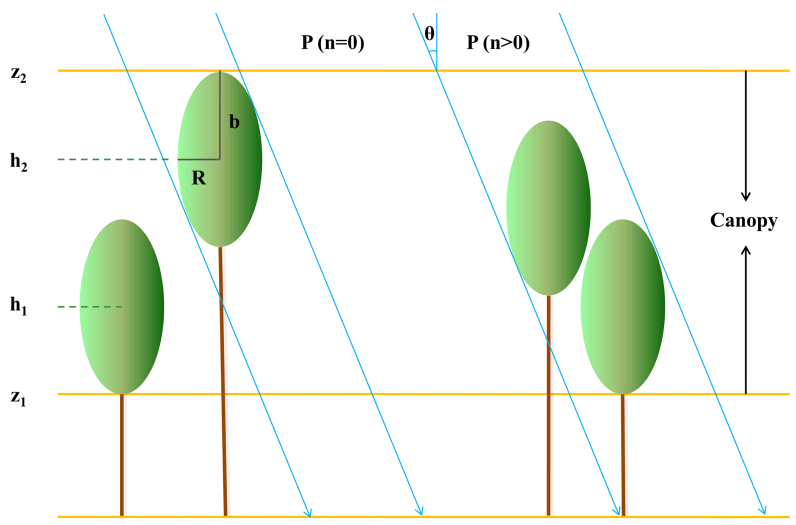
\includegraphics[width=0.5\textwidth]{/home/mn811042/Thesis/chapter4/figures/GORT_schematic.png}
        \caption{A scheme of the canopy structure in the Geometric Optical Radiative Transfer model as modified from \citet{Ni1998}.} 
\label{fig:gort_scheme}
\end{figure}

Gap probability, or direct transmittance, is the probability of photons reaching a given vegetation canopy depth without being intercepted by plant elements. It is a key variable to characterise the radiation partitioning within vegetation canopies. A detailed description for modelling the gap probability with GORT is described in previous studies \citep{Li1995,Ni1999}, in here the concept of gap probability is briefly summarised. For  homogeneous  canopies,  Beer\textsc{\char13}s  law  describes  the gap  probability  of  sunlight  penetration, while for discontinuous plant canopies, leaves are clumped within individual canopy crowns, creating an uneven distribution of gap probabilities for beam radiation.

The goals of this section are to: 
\begin{enumerate}
\item explore the differences in absorbance, reflectance and transmittance in the PAR spectrum (400 - 700 nm) related to a series of variables: structural (lower and upper boundary of the crown centres, tree density, vertical and horizontal crown radius and their ratio, and crown shape), geometrical (leaf angle distributions following \citet{deWit1965} and solar zenith angle), spectral (leaf and soil albedo) and optical (leaf area index, analogous to the optical depth of a canopy); and 

\item evaluate how the parameters $a$ and $b$ of the structure factor parameterisation \citep{pinty2006} varies with the same evaluated variables. 
A default canopy with LAI = 1.0 m$^2$.m$^{-2}$ and canopy cover of 20\% was set for this exercise and it is described in details in Table~\ref{tab:parameters_gort}. For all evaluated variables, the other ones were fixed on a base value and they varied in a pre-defined range. Except for the case of vertical to horizontal crown radius ratio (b/R), where they varied together following the range between 10$^{-3}$ to 10$^2$.
\end{enumerate}
\begin{threeparttable}
\centering
\caption{Base values and ranges for parameters used in GORT.}
%\begin{tabular*}{\textwidth}{ l@{\extracolsep{\fill}}*{4}{c}}
\begin{tabular}{lP{0.20\textwidth} lP{0.25\textwidth} lP{0.25\textwidth} lP{0.25\textwidth}}
%\begin{tabular}{\textwidth}{|p{\textwidth/4}|p{\textwidth/4}|p{\textwidth/4}|p{\textwidth/4}|}
%\begin{tabular*}
     \hline
     \hline
\textbf{Parameter}   & \textbf{Description} & \textbf{Base Value (Unit)} & \textbf{Range} \\
\noalign{\smallskip}\hline
$h_1$          & Lower boundary of the crown centres       & 7.0  (0.01) m & 0.01 - 49.9 \\
$h_2$          & Upper boundary of the crown centres       & 11.0  (50) m & 0.02 - 50.0 \\
$\lambda$         & Tree density                              & 40 trees/ha &  1 - 1000\\
$b$            & Vertical crown radius                     & 5 m & 0 - 50\\ 
$R$            & Horizontal crown radius                   & 5 m &  0 - 50\\
$b/R$           & Vertical to horizontal crown radius ratio & 1 & 10$^{-3}$ - 10$^2$\\
SZA            & Solar Zenith angle                        & 45$^{\circ}$ & 0$^{\circ}$ - 90$^{\circ}$ \\
LAI            & Leaf Area Index                           & 1.0 m$^2$.m$^{-2}$ &  0.1 - 10.0\\
$\omega$           & Leaf single scattering albedo             & 0.13 &  0.00 - 1.00\\
$\alpha_{soil}$  & Soil albedo                               & 0.12 & 0.00 - 1.00\\ 
LAD$^*$             & G-function                                & Spherical & \citet{deWit1965} \\
Shape$^*$           & Crown shape                               & Round & \citet{Duursma2012} \\
\hline
\hline\noalign{\bigskip}
%\end{tabular*}
\end{tabular}
\begin{tablenotes}
      \small
      \item $^*$ The evaluations highlighted were performed with the MAESPA model instead of GORT
            simply because of availability.  
\end{tablenotes}
\label{tab:parameters_gort}
\end{threeparttable}

%/home/mn811042/Thesis/chapter4/experiment1/gort/balance_h1.pdf

\begin{figure}
\centering

\begin{tabular}{lll}
\subfloat[$h_1$]{\includegraphics[trim=0cm 0cm 0cm 0cm,angle=0,clip=true,width=0.33\textwidth]{/home/mn811042/Thesis/chapter4/experiment1/gort/balance_h1.png}}
&
\subfloat[$h_2$]{\includegraphics[trim=0cm 0cm 0cm 0cm,angle=0,clip=false,width=0.33\textwidth]{/home/mn811042/Thesis/chapter4/experiment1/gort/balance_h2.png}}
&
\subfloat[$\lambda$]{\includegraphics[trim=0cm 0cm 0cm 0cm,angle=0,clip=false,width=0.33\textwidth]{/home/mn811042/Thesis/chapter4/experiment1/gort/balance_lambda.png}}
&
\end{tabular}

\begin{tabular}{lll}
\subfloat[$b$]{\includegraphics[trim=0cm 0cm 0cm 0cm,angle=0,clip=false,width=0.33\textwidth]{/home/mn811042/Thesis/chapter4/experiment1/gort/balance_b.png}}
&
\subfloat[$R$]{\includegraphics[trim=0cm 0cm 0cm 0cm,angle=0,clip=false,width=0.33\textwidth]{/home/mn811042/Thesis/chapter4/experiment1/gort/balance_r.png}}
&
\subfloat[$b/R$]{\includegraphics[trim=0cm 0cm 0cm 0cm,angle=0,clip=false,width=0.33\textwidth]{/home/mn811042/Thesis/chapter4/experiment1/gort/balance_b_r_ratio.png}}
\end{tabular}

\begin{tabular}{lll}
\subfloat[LAI]{\includegraphics[trim=0cm 0cm 0cm 0cm,angle=0,clip=false,width=0.33\textwidth]{/home/mn811042/Thesis/chapter4/experiment1/gort/balance_lai.png}}
&
\subfloat[$\omega$]{\includegraphics[trim=0cm 0cm 0cm 0cm,angle=0,clip=false,width=0.33\textwidth]{/home/mn811042/Thesis/chapter4/experiment1/gort/balance_omega.png}}
&
\subfloat[$\alpha_{soil}$]{\includegraphics[trim=0cm 0cm 0cm 0cm,angle=0,clip=false,width=0.33\textwidth]{/home/mn811042/Thesis/chapter4/experiment1/gort/balance_albs.png}}
\end{tabular}

\begin{tabular}{lll}
\subfloat[Crown shape]{\includegraphics[trim=0cm 0cm 0cm 0cm,angle=0,clip=false,width=0.33\textwidth]{/home/mn811042/Thesis/chapter4/experiment1/maespaenv/balance_crown.png}}
&
\subfloat[LAD]{\includegraphics[trim=0cm 0cm 0cm 0cm,angle=0,clip=false,width=0.33\textwidth]{/home/mn811042/Thesis/chapter4/experiment1/maespaenv/balance_LAD.png}}
&
\subfloat[SZA]{\includegraphics[trim=0cm 0cm 0cm 0cm,angle=0,clip=false,width=0.33\textwidth]{/home/mn811042/Thesis/chapter4/experiment1/gort/balance_sza.png}}
\end{tabular}

\caption{PAR partitioning in three radiative components: absorbance (red), reflectance (blue) and transmittance (green) for 12 different structural, geometrical, spectral or optical variables generated with the GORT and MAESPA models}
\label{f:balance_gort}
\end{figure}

Fig.~\ref{f:balance_gort} presents the results in terms of the “term of the radiation partitioning” on the y-axis (absorbance, reflectance and transmittance) versus each one of the evaluated variables. 

For $h_1$ and $h_2$ the tested values are indicated by parentheses. In the first case $h_1$ varied from 0.01 to 49.9 meters with $h_2$ fixed on 50.0 meters. In the second case $h_1$ was fixed on a constant value equals to 0.01 m and $h_2$ varied from 0.02 to 50.0 meters. In both cases the effect of boundary of the crown centres on radiation partitioning was negligible. The results indicates that the position of crown centres does not affect mutual shadowing when everything else is set to be constant.

Tree stem density varied from 1 to 1000 trees per hectare and seemed to have a significant impact on radiation partitioning in three distinct behaviors. The first thing to be noticed when the number of trees increases is an abrupt increase in PAR absorption, because there is more vegetation elements in the evaluated area, but still lots of empty spaces, so no mutual shadowing is observed. As soon as the number of trees gets closer to 100, the value of PAR absorption presents a slightly decrease, followed by an increase in direct transmittance and reflectance. The total LAI of the area was set to be constant and equals to 1.0 m$^2$.m$^{-2}$, so in order to keep the same LAI the within-crown gaps increase, even though the between-crown gaps are decreasing the total amount of gap probability increases. After a local maximum in gap probability associated with approximately 450 trees per hectare the third and last behavior of radiation partitioning with tree density is a constant decrease in direct transmittance and reflectance and an increase in PAR absorption. Mathematically the area occupied by the ellipsoidal trees is now 3.5 times bigger than the total area and both type of gaps - between and within crown - decrease. For the evaluated range of tree densities PAR absorption varied in about 60\%, as well as PAR direct transmittance and reflectance varied at the order of 5\%.

Fig.~\ref{f:balance_gort} also indicates that both vertical and horizontal crown radius and their respective ratio have a large impact on radiation partitioning. An increase in vertical crown radius from about 0 to 50 m increases mutual crown shadowing and decreases within-crown gaps. In the evaluated range (0 - 50 m), the direct transmissivity decreased by 60\%, followed by an increase of the same magnitude in absorption and a decreased of about 10\% in reflectance. 

Although the horizontal crown radius also presented a substantial impact on radiation partitioning, different patterns in the curve indicate different responses of radiation partitioning related to certain values of horizontal crown radius, or more generally to the ratio between vertical and horizontal crown radius. 

The first identifiable pattern on the radiation partitioning is an abrupt increase in the order of 40\% in radiation absorption and a decrease of the same order in direct transmittance and in reflectance about 5\%. This behavior can be observed until horizontal crown radius is about the order of 10 m, or double the size of the vertical radius. After that, the second observed pattern is the opposite than the first one, but not as strong as the previous one. When the horizontal crown radius is from approximately the order of 10 to 20 m, or twice to four times the size of the vertical crown radius, the radiation absorption goes through a decrease of approximately 25\%, as well as the gap probability increases as much, and reflectance increases by 10\%. These behaviors can be explained by the increase of within-crown gaps. The third pattern is exactly as the first one, as the total gap probability decreases, but at this time in the order of approximately 60\%, followed by an increase of the same order in PAR absorption and a decrease of about 15\% in reflectance. This third pattern is observed when horizontal crown radius is in the range of approximately 20 to 30 m, or 4 to 6 times larger than the vertical crown radius. At the end of the evaluated range (R $>$ 30 m), the radiation partitioning reaches a plateau, where absorption represents approximately 90\% of the total radiation. The same type of behavior can be observed when analyzing the ratio between vertical and horizontal crown radius. These results indicate a strong influence of crown shape in radiation partitioning and points to the importance of appropriately characterizing and taking into account the effects of crown vertical and horizontal radius on radiative transfer in vegetation canopies.
   
In this experiment the LAI was also varied from 0.1 to 10 m$^2$.m$^{-2}$, with everything else fixed. The effects of LAI on radiation partitioning for the evaluated canopy reached a saturation by LAI = 2.0 m$^2$.m$^{-2}$ and the total variation in radiation partitioning was limited to 15\% more PAR absorption. Higher LAI only changes the within-crown gaps in this case, and according to this analysis, doubling the LAI is already enough to saturate the signal in changes on radiation partitioning. 

Regarding the canopy spectral properties, the overall changes in radiation partitioning followed by changes in the leaf single scattering albedo ($\omega$) were limited to about 10\% for absorption, slightly lower for reflectance and almost no changes were observed in transmittance. The leaf single scattering albedo is defined as the sum of the leaf transmittance ($\tau$) and the leaf reflectance ($\rho$), both in the PAR spectral region, and the evaluated range for $\omega$ was between 0.0 and 1.0. Changes in absorption are linearly anti-correlated to $\omega$ and the opposite is observed for reflectance. As $\omega$ increases, there is more scattering associated with it and more radiation leaves the canopy without being absorbed. 

Even though this effect can be observed, it is not as strong as the effects of soil albedo on radiation partitioning. In this sensitivity analysis, the same type of procedure was conducted with soil albedo ($\alpha_{soil}$) varying between 0.0 and 1.0. The results indicate a large impact of the order of 60\% on canopy reflectance and 20\% on canopy absorption. 

On the contrary of what is observed when leaf albedo increases, the soil albedo has a positive effect on canopy absorption because the soil reflects backwards the direct transmitted downwelling radiation and increases the probability of the same radiation, now going upwards after going through scattering processes, being reabsorbed by plants. Direct transmittance is not affect by soil albedo. In general, spectral properties greatly influence radiation partitioning and have to be taken into account when calculating radiative transfer in plant canopies.

The structure of a tree crown is defined as the spatial and angular distributions of all phytoelements (leaves, twigs, branches, stems, etc.) and their sizes and shapes within the tree crown \citep{Wang1990a}. In order to evaluate another two different elements of canopy structure not covered by GORT: crown shape other than ellipsoids and leaf angle distribution, the MAESPA model was used in the simulations. 

Perhaps the most important feature of the MAESPA model is the level of detail it uses to represent a plant canopy \citep{Medlyn2004}. The radiation routines are described in detail by \citet{Wang1990}. The canopy consists of individual tree crowns, which are described by a basic shape of the crown including: conical, half-ellipsoidal, paraboloidal, full-ellipsoidal, upright cylinder and even a “box” shape (suitable for the mini-ecosystems, for example). The default of the model is half-ellipsoidal (Fig.~\ref{f:crown_shapes}).

\begin{figure}
\centering

\begin{tabular}{lll}
\subfloat[Round]{\includegraphics[height=5cm,width=0.3\textwidth]{/home/mn811042/Thesis/chapter4/experiment1/maespaenv/crownshape/round_2.png}}
&
\subfloat[Cone]{\includegraphics[height=5cm,width=0.3\textwidth]{/home/mn811042/Thesis/chapter4/experiment1/maespaenv/crownshape/cone_2.png}}
&
\subfloat[Cylinder]{\includegraphics[height=5cm,width=0.3\textwidth]{/home/mn811042/Thesis/chapter4/experiment1/maespaenv/crownshape/cylinder_2.png}}
\end{tabular}

\begin{tabular}{lll}
\subfloat[Ellipsoid]{\includegraphics[height=5cm,width=0.3\textwidth]{/home/mn811042/Thesis/chapter4/experiment1/maespaenv/crownshape/elipsoid_2.png}}
&
\subfloat[Half-ellipsoid]{\includegraphics[height=5cm,width=0.3\textwidth]{/home/mn811042/Thesis/chapter4/experiment1/maespaenv/crownshape/halfellipsoid_2.png}}
&
\subfloat[Paraboloid]{\includegraphics[height=5cm,width=0.3\textwidth]{/home/mn811042/Thesis/chapter4/experiment1/maespaenv/crownshape/paraboloid_2.png}}
\end{tabular}

\subfloat[MAESPA canopy representation]{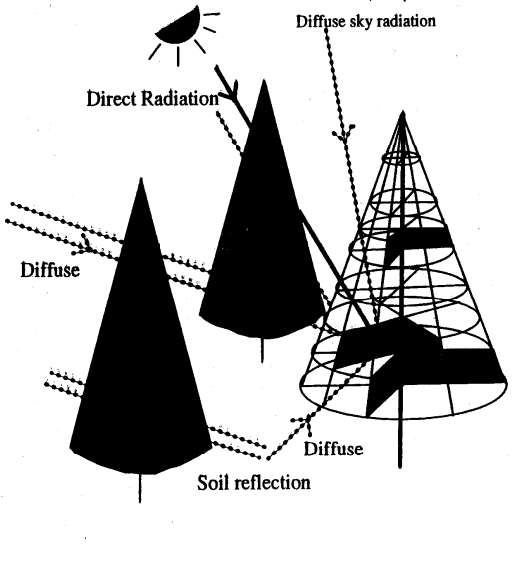
\includegraphics[width=0.5\textwidth]{/home/mn811042/Thesis/chapter4/figures/cone_MAESPA.png}}
        
\caption{Representation of available crown shapes in MAESPA (a - f), except for ``box'', and a conical canopy representation in MAESPA from \citet{Medlyn2004} (g).}
\label{f:crown_shapes}
\end{figure}


A number of grid points are located in a target crown and radiation at those grid points is calculated based on shading within the crown, shading by neighbouring trees, the solar zenith ($\theta$ = 45$^{\circ}$) and azimuth ($\phi$ = 0$^{\circ}$) angle and whether radiation is direct or diffuse (Fig.~\ref{f:crown_shapes}). Scattering of radiation is approximated following \citet{Norman1979}. 

Previous studies \citep{Oker-Blom1982,Kuuluvainen1987} showed that there were small differences (less than 5\%) in absorbed PAR by crowns of a reasonably wide range of ellipsoidal shapes. In this sensitivity analysis, the differences in absorbed PAR between different crown shapes were limited to about 10\% between a box (fAPAR$_{box}$ = 0.26) and a conical (fAPAR$_{cone}$ = 0.15) shape. All the other crown shapes presented values of fraction of absorbed PAR of the order of 0.24. 

The conical crown shaped canopy also showed an approximately 17\% higher direct transmittance in comparison to the uniform box shape and a decrease in reflectance. This is a relevant result to be taken into account in boreal coniferous forests, for example. These forests usually present increased soil albedo during winter in the presence of snow and a substantial mutual shadowing between the needles of a shoot. An increased direct transmittance associated with a conical crown shape in the presence of snow could result in even more backscattered radiation, and more PAR absorption. These regions of the world are light limited in great part of the year and this behaviour could help trees to absorb more radiation.  
  
The same idea of exploring different structural properties can be applied to leaf angle distributions. For this experiment, the leaf angle distribution (G-function) within crowns was written following six special probability distribution functions ($g^{\prime}(\theta_l)$)  described by \citet{deWit1965}: (i) \textit{spherical} or random, where the relative frequency of leaf angle is the same as for surface elements of a sphere; (ii) \textit{planophile}, where horizontal leaves are most frequent; (iii) \textit{erectophile}, where vertical leaves are most frequent; (iv) \textit{plagiophile}, where oblique ($\theta_l$ $\approx$ 45$^{\circ}$) leaves are most frequent, (v) \textit{extremophile}, where oblique leaves are least frequent, i.e., mostly horizontal or vertical leaves; and (vi) \textit{uniform}, where the proportion of leaf angle is the same at any angle (Fig.~\ref{f:g_function}). 

\begin{figure}[ht]
      	\centering
        \includegraphics[width=1\textwidth]{/home/mn811042/src/pySellers/g_function.png}
        \caption{Leaf angle distribution function is described as the proportion of leaves ($g^{\prime}(\theta_l)$ function) for different angles.} 
\label{f:g_function}
\end{figure}

In MAESPA the leaf angle distribution used in the radiative transfer calculations can be specified by:

(a) the number of leaf angle classes (N$\alpha$) and the ratio of the horizontal and vertical axes of an ellipsoid ($\chi$), which is the parameter of an ellipsoidal leaf angle distribution \citep{Campbell1990}. If N$\alpha$ = 1, there is only one leaf angle class with an average angle ($\overline{\theta_l}̅$). If N$\alpha$ $>$ 1, ($\overline{\theta_l}̅$) is used to generate the leaf inclination angle distribution assuming an elliptical distribution.

(b) If $\chi$ = 1, the distribution is spherical; if $\chi$ = 0.5, the distribution is erectophile; and if $\chi$ = 2, the distribution is planophile. 

(c) Alternatively, the proportion of leaf area in each angle class can be read from an array (F$\alpha$). 

MAESPA can take up to nine possible leaf angle classes and the distribution of angles is elliptical following the parameter $\chi$. The default is N$\alpha$ = 1 and $\chi$ = 1, i.e. one leaf angle class, spherical distribution. 

For the particular evaluated canopy, the leaf angle distribution (G-function) caused a difference of up to 4\% in absorbed PAR, 17\% in direct transmitted PAR and less than 1\% in reflectance. The biggest difference caused by the G-function on radiation partitioning was between the erectophile and planophile distributions as expected once these two distributions are the opposite. 

A canopy with most leaves in the vertical position (erectophile) allows more radiation goes through it with fewer interactions (fAPAR = 0.25) than a canopy with most leaves in the horizontal position (planophile), which blocks more direct light and presents more absorption (fAPAR = 0.29). All the other distributions are somewhere in between these two. 

Finally, the geometrical impact on radiation partitioning due to the position of the Sun in the sky is well understood  and described by the radiative transfer theory, but still needs to be explored when analysing it over open forest canopies with heterogeneous structural features.

The position of the Sun in relation to the zenith (the point in the sky or celestial sphere directly above an observer) gives the so called solar zenith angle and describes the position in which the Sun is located in the celestial sphere. In order to have a precise position of the Sun, the observer needs a combination of two different types of information: first the Solar Zenith angle, and second the Solar azimuth angle, defined as the position of the sun in relation to the North, where 0 degrees indicates the Sun is in the North. In this case, azimuthal variations were excluded of the analysis, because the optical depth of a vegetation canopy is mostly affected by zenithal variations. 

When the source of radiation is right above a heterogeneous canopy, the radiation has less material to interact in the presence of more gaps. As the solar zenith angle increases the path length of the radiation increases and because there is more material in this path length the optical depth of the canopy increases as well. This effect can be observed by the radiation partition evaluated in Fig.~\ref{f:balance_gort} with solar zenith angle varying. The direct transmittance decreases because the between-crown gaps are less observable in high solar zenith angles, and the direct transmittance is mainly caused by within-crown gaps. As the direct transmittance decreases the absorption increases because there is more plant elements being illuminated. Finally, the reflectance also decreases because there is less direct radiation reaching the soil and being scattered isotopically with lower intensity.

For this specific canopy in proportional terms, radiation absorption peaks when the solar zenith angle is around 85$^{\circ}$ in 60\%, as well as transmittance decreases to a minimum of around 40\%. The variation in both terms for all possible solar zenith angles (0$^{\circ}$ - 90$^{\circ}$) is of about 35\%. Reflectance goes from about 10\% in when the solar zenith angle is 0$^{\circ}$ to about half of that by 85$^{\circ}$. The extreme end of the zenith angles possibilities, from approximately 85$^{\circ}$ to 90$^{\circ}$ has a different behaviour from the rest of the curve mainly because of edge effects. If the canopy was infinite, or the crown centres were immediately close to the ground this effect could be minimised. 

Indeed angular variations are one of the most important variables when studying radiative transfer in forest canopies, especially heterogeneous ones. The idea behind a factor that accounts for structural effects of vegetation on radiation partitioning is well accepted by the scientific community and often taken into account when calculating radiative transfer for different purposes. However, the angular variation of this ``correction factor'' is still an open debate and needs to be further explored. 

As discussed before, the presence of an angular dependence on clumping index, or in here referred as the ‘structure factor’ following \citet{pinty2006}, could improve considerably the radiation partitioning of simpler 1D radiative transfer models because structural canopy features depend on observation or incident radiation angles. 

First, the following section explore the same sensitivity analysis developed in here, but at this time through an index proposed by \citet{Hoffman1983} in order to mathematically characterise the impact of each of the evaluated variables on the radiation partitioning in 3D radiative transfer models. 

\subsection{`Local' sensitivity analysis of related canopy radiative transfer variables}
Usually authors \citep{Downing1985,Iman1988} use the terms `sensitive', `important', `most influential', `major contributor', `effective', or `correlated' interchangeably to refer to the degree to which an input parameter affects the model output \citep{Hamby1994}.

\citet{Crick1987} have made a distinction by referring to 'important' parameters as those whose uncertainty contributes substantially to the uncertainty in assessment results, and 'sensitive' parameters as those which have a significant influence on assessment results. The consensus among authors is that models are indeed sensitive to input parameters in two distinct ways: (1) the variability, or uncertainty, associated with a sensitive input parameter is propagated through the model resulting in a large contribution to the overall output variability, and (2) model results can be highly correlated with an input parameter so that small changes in the input value result in significant changes in the output \citep{Hamby1994}.

Conceptually, the simplest method to perform a sensitivity analysis is to repeatedly vary one parameter at a time while holding the others fixed \citep{Downing1985,Crick1987}. A sensitivity ranking can be obtained quickly by increasing each parameter by a given percentage while leaving all others constant, and quantifying the change in model output. This type of analysis has been referred to as a 'local' sensitivity analysis \citep{Crick1987} since it only addresses sensitivity relative to the point estimates chosen and not for the entire parameter distribution. 

A simple method of determining parameter sensitivity is to calculate the output percentage difference when varying one input parameter from its minimum value to its maximum value \citep{Hoffman1983,Bauer1991}. \citet{Hoffman1983} advocate utilising each parameter's entire range of possible values in order to assess true parameter sensitivities. The 'sensitivity index' (SI) is calculated using,
\begin{equation}
SI = \frac{D_{max}-D_{min}}{D_{max}}
\label{equation:si}
\end{equation}
\noindent where $D_{min}$ and $D_{max}$ represent the minimum and maximum output values, respectively, resulting from varying the input over its entire range \citep{Hoffman1983}. This figure-of-merit provides a good indication of parameter and model variability.

\begin{figure}
\centering
\begin{tabular}{lll}
\subfloat[Absorption]{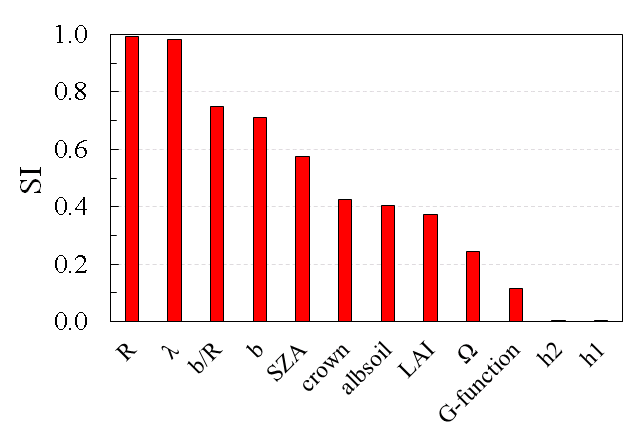
\includegraphics[width=0.3\textwidth]{/home/mn811042/Thesis/chapter4/figures/SI_absorbance.png}}
&
\subfloat[Reflectance]{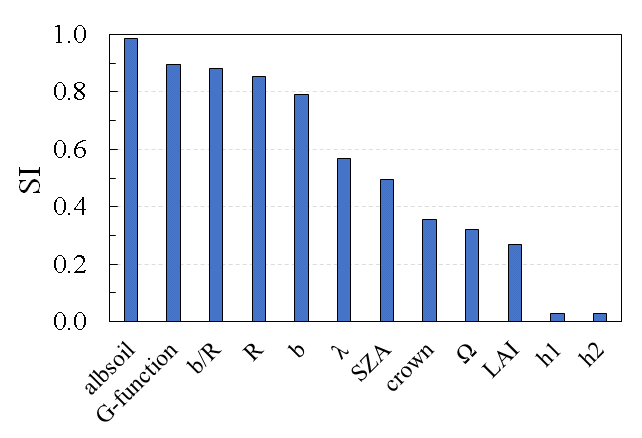
\includegraphics[width=0.3\textwidth]{/home/mn811042/Thesis/chapter4/figures/SI_reflectance.png}}
&
\subfloat[Transmittance]{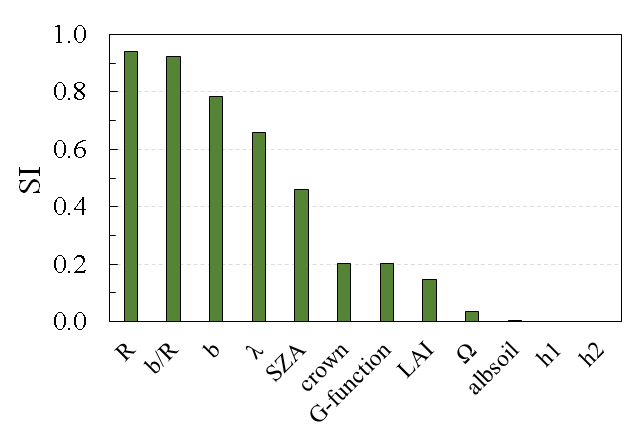
\includegraphics[width=0.3\textwidth]{/home/mn811042/Thesis/chapter4/figures/SI_transmittance.png}}
\end{tabular}
\caption{‘Local’ sensitivity analysis of 12 parameters described in Table~\ref{tab:parameters_gort} through the evaluation of the ‘Sensitivity Index’ (SI) \citep{Hoffman1983} for terms of the radiation partitioning of PAR a) absorption, b) reflectance and c) transmittance.}
\label{f:si_radiationpartitioning}
\end{figure}

Fig.~\ref{f:si_radiationpartitioning} shows the sensitivity index for 12 parameters related to canopy structure, geometry, spectral and optical properties detailed described in Table~\ref{tab:parameters_gort}. As the analysis performed in the previous section, the sensitivity index rank the variables from 0, which indicates the model results are not well correlated with an input parameter and 1, which indicates high correlated parameters, so that small changes in the input value result in significant changes in the terms of the PAR radiative partitioning evaluated with the models GORT and MAESPA. 

In terms of absorption, Fig.~\ref{f:si_radiationpartitioning}a indicates that the parameters $R$, horizontal crown radius, and λ, tree density, are responsible for the major changes, followed by two other structural variables, $b/R$ and $b$. The `local' sensitivity analysis reinforce the fact that canopy structure is the most important factor influencing PAR absorption. Solar zenith angle (SZA) comes in fourth place and indicates a strong influence of Sun geometry. 

The same type of behaviour is observed when analysing transmittance (Fig.~\ref{f:si_radiationpartitioning}c), where the most influential variables are the ones related to canopy structure, followed by the position of the radiation source. The difference however is related to the fact that crown ellipsoidal shape defined by horizontal crown radius, the vertical to horizontal crown radius ratio and the vertical crown radius are more influent over transmittance than tree density itself. 

In terms of canopy albedo, or reflectance (Fig.~\ref{f:si_radiationpartitioning}b), the soil albedo is the most influential parameter. It is important to highlight the vegetation canopy cover of 20\% when evaluating canopy albedo. That means 80\% of the scene is bare soil and because of that, the soil albedo is very impacting on canopy reflectance. This result would be probably different if the evaluated canopy was denser with higher canopy cover.

Perhaps one of the most important things to take from the analysis performed here is the fact that solar zenith angle has always a greater impact than LAI for the three terms of the radiation partitioning, absorption, reflectance and transmittance. The LAI is frequently used in 1D radiative canopy models as a parameter to determine the optical depth of a homogeneous canopies. But is the LAI a sufficient parameter to describe the optical depth of a real heterogeneous forest canopy? The next section explores the ability of LAI in taking into account structural heterogeneities on radiative partitioning. 

\subsection{Can LAI take into account vegetation canopy structural variabilities?}
Even though a large number of advances were used to improve canopy radiative transfer models, the most impacting variable to prescribe the radiative transfer in current models is the leaf area index, or the LAI \citep{Yang2001}. The typical values of LAI can vary from 1 to 9 m$^2$.m$^{-2}$ for a broadleaf forest, or from 1 to 3 for scrubs \citep{Clark2011}. In order to identify variations in predicted fraction of absorbed PAR (fAPAR) related to different factors associated with canopy structure, a more specific sensitive analysis was conducted based on a previous experiment proposed by \citet{pinty2006} for three different vegetation conditions (Fig.~\ref{f:3d_maespa}), using a 1D radiative transfer model where the vegetation canopy is treated as turbid medium model, Two-Stream scheme \citep{Sellers1985}, and a 3D radiative tree based model, MAESPA \citep{Duursma2012}, with a fixed value of LAI of 3.2 m$^2$.m$^{-2}$ and a range of different parameters set up as described in Table~\ref{tab:parameters_laisense}.

\begin{threeparttable}
\centering
\caption{Variables Defining the Structurally Heterogeneous Scenes.}
%\begin{tabular*}{\textwidth}{ l@{\extracolsep{\fill}}*{4}{c}}
\begin{tabular}{l{0.25\textwidth} l{0.75\textwidth}}
%\begin{tabular}{\textwidth}{|p{\textwidth/4}|p{\textwidth/4}|p{\textwidth/4}|p{\textwidth/4}|}
%\begin{tabular*}
     \hline
     \hline
\textbf{Variable Identification}   & \textbf{Values (Units)}\\
\noalign{\smallskip}\hline
Mean Leaf Area Index over the domain         &	3.19$^S$, 3.19$^M$ and 3.15$^D$ (m$^2$.m$^{-2}$)\\
Mean Leaf Area Index of a single tree crown  &	6.02$^S$, 2.25$^M$ and 0.21$^D$ (m$^2$.m$^{-2}$)\\
Tree density 	                             & 53$^S$, 142$^M$ and 4718$^D$ (trees/ha)\\
Mean tree height	                     &23.99$^S$, 24.49$^M$ and 9.92$^D$ (m)\\
Mean tree crown height	                     &7.59$^S$, 7.09$^M$ and 7.57$^D$ (m)\\
Spatial distribution of tree locations	     & Random distribution\\
Crown shape	                             & Ellipsoid\\
Soil reflectance$^a$	                     & 0.100\\
Leaf reflectance$^a$	                     & 0.082\\
Leaf transmittance$^a$ 	                     & 0.093\\
\hline
\hline%\noalign{\bigskip}
%\end{tabular*}
\end{tabular}
\begin{tablenotes}
      \small
      \item $^S$Sparse vegetation. $^M$Medium vegetation. $^M$Dense vegetation. 
      \item $^a$ PAR wavelength. 
\end{tablenotes}
\label{tab:parameters_laisense}
\end{threeparttable}

\bigskip

\begin{figure}
\centering
\begin{tabular}{ll}
\subfloat[Sparse Canopy]{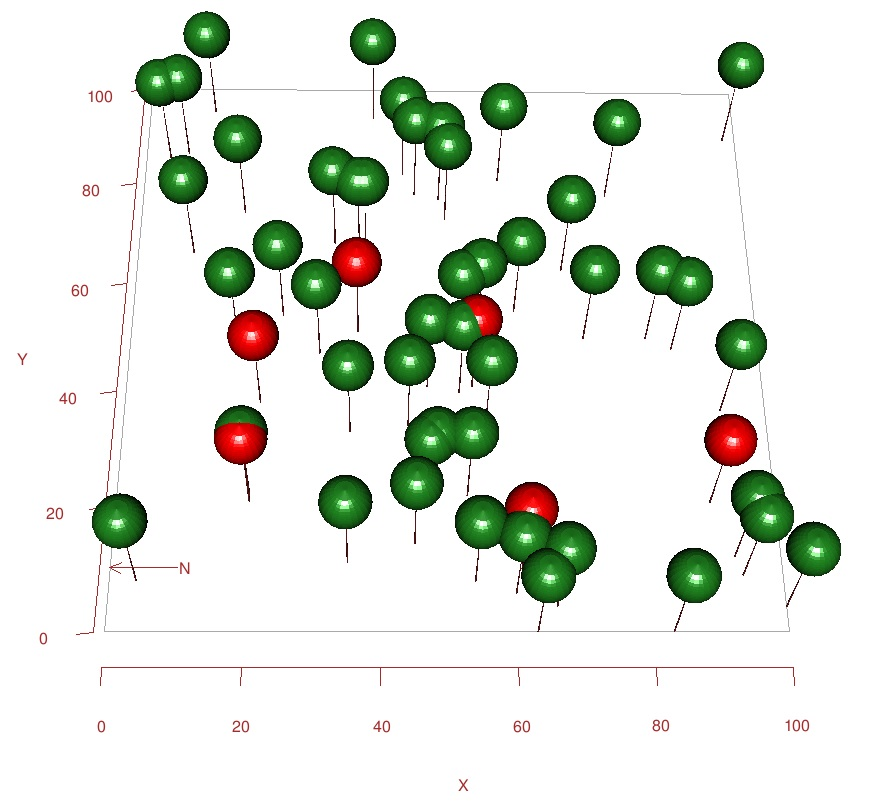
\includegraphics[width=0.4\textwidth]{/home/mn811042/Thesis/chapter4/figures/sparse_1.png}
                         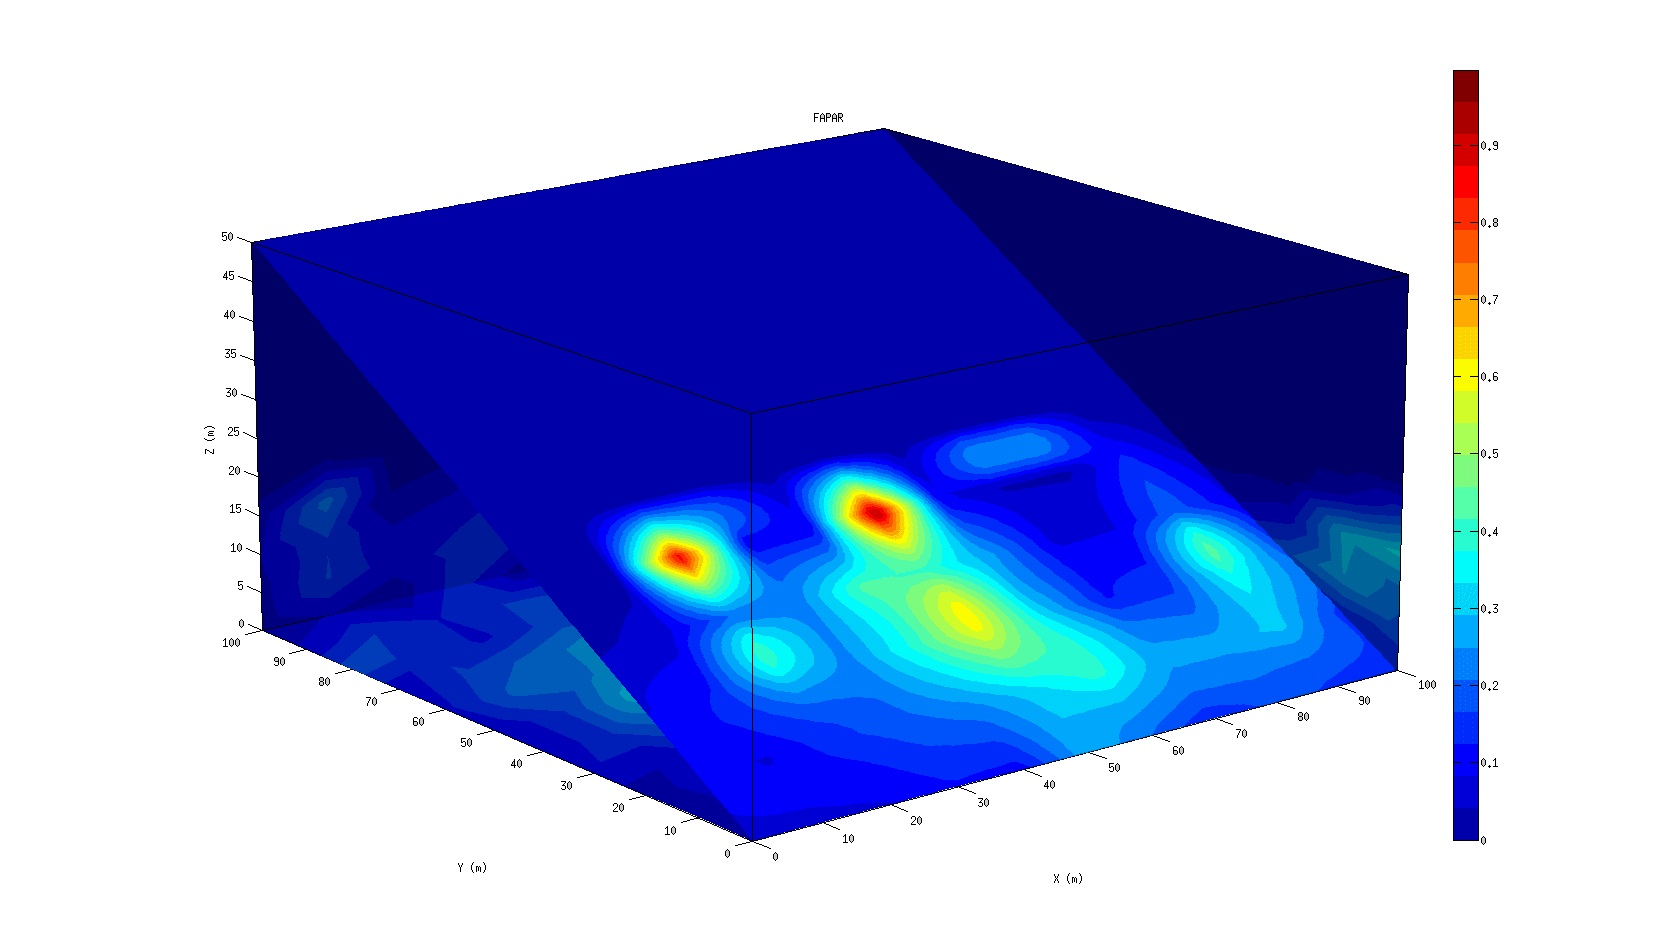
\includegraphics[width=0.6\textwidth]{/home/mn811042/Thesis/chapter4/figures/FAPAR_sparse.png}}
\end{tabular}

\begin{tabular}{ll}
\subfloat[Medium Canopy]{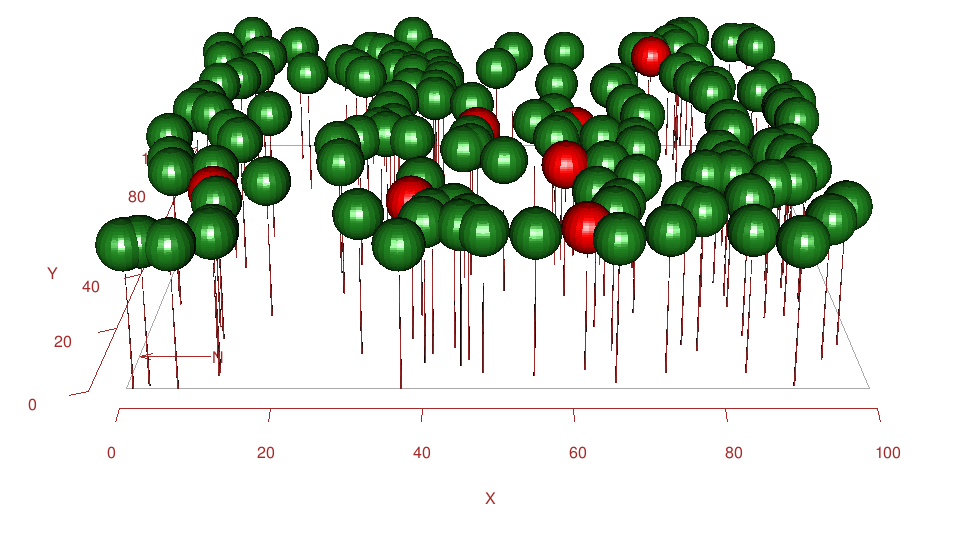
\includegraphics[width=0.4\textwidth]{/home/mn811042/Thesis/chapter4/figures/medium_1.png}
                         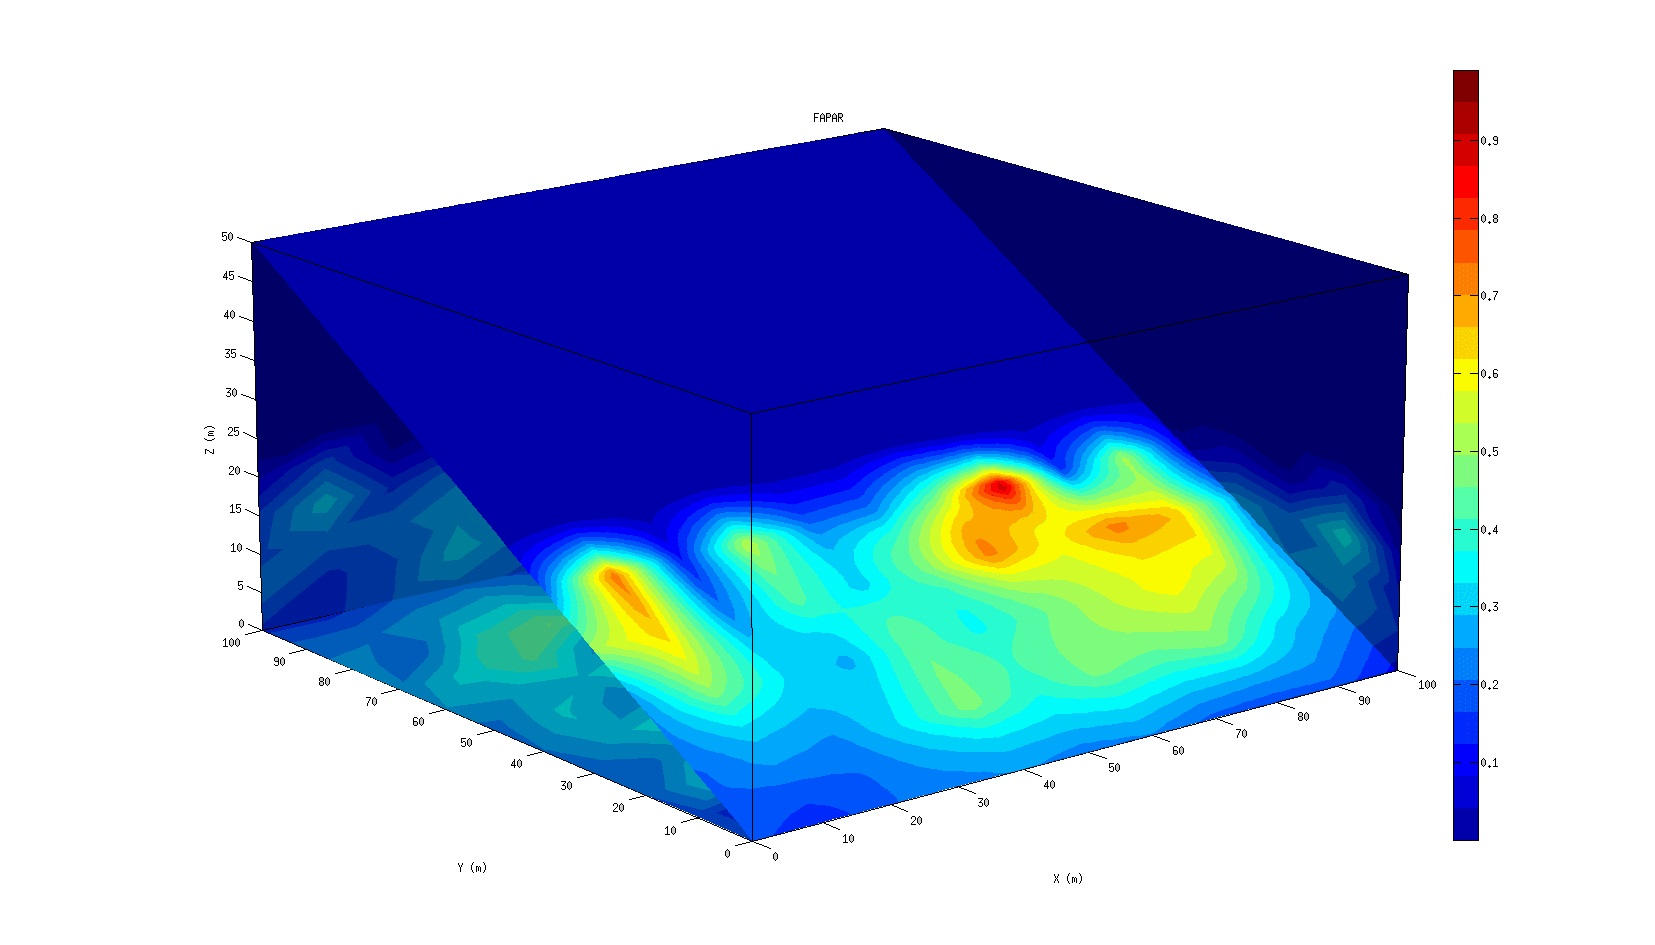
\includegraphics[width=0.6\textwidth]{/home/mn811042/Thesis/chapter4/figures/FAPAR_medium.png}}
\end{tabular}

\begin{tabular}{ll}
\subfloat[Dense Canopy]{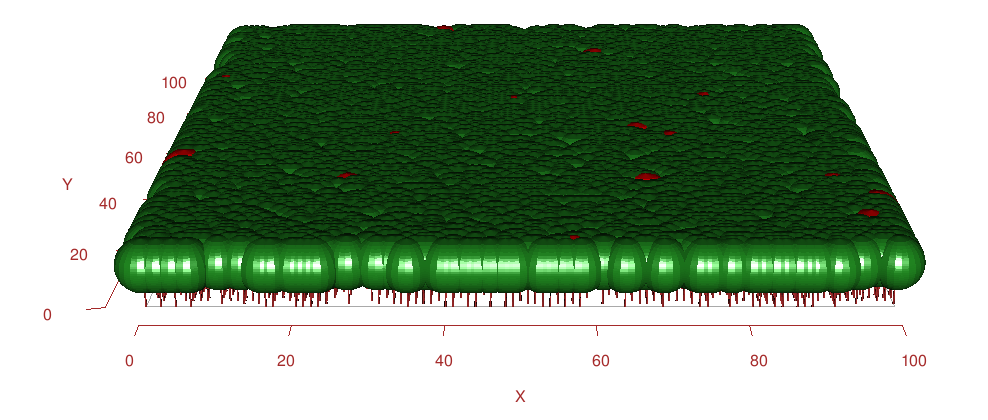
\includegraphics[width=0.4\textwidth]{/home/mn811042/Thesis/chapter4/figures/dense_1.png}
                        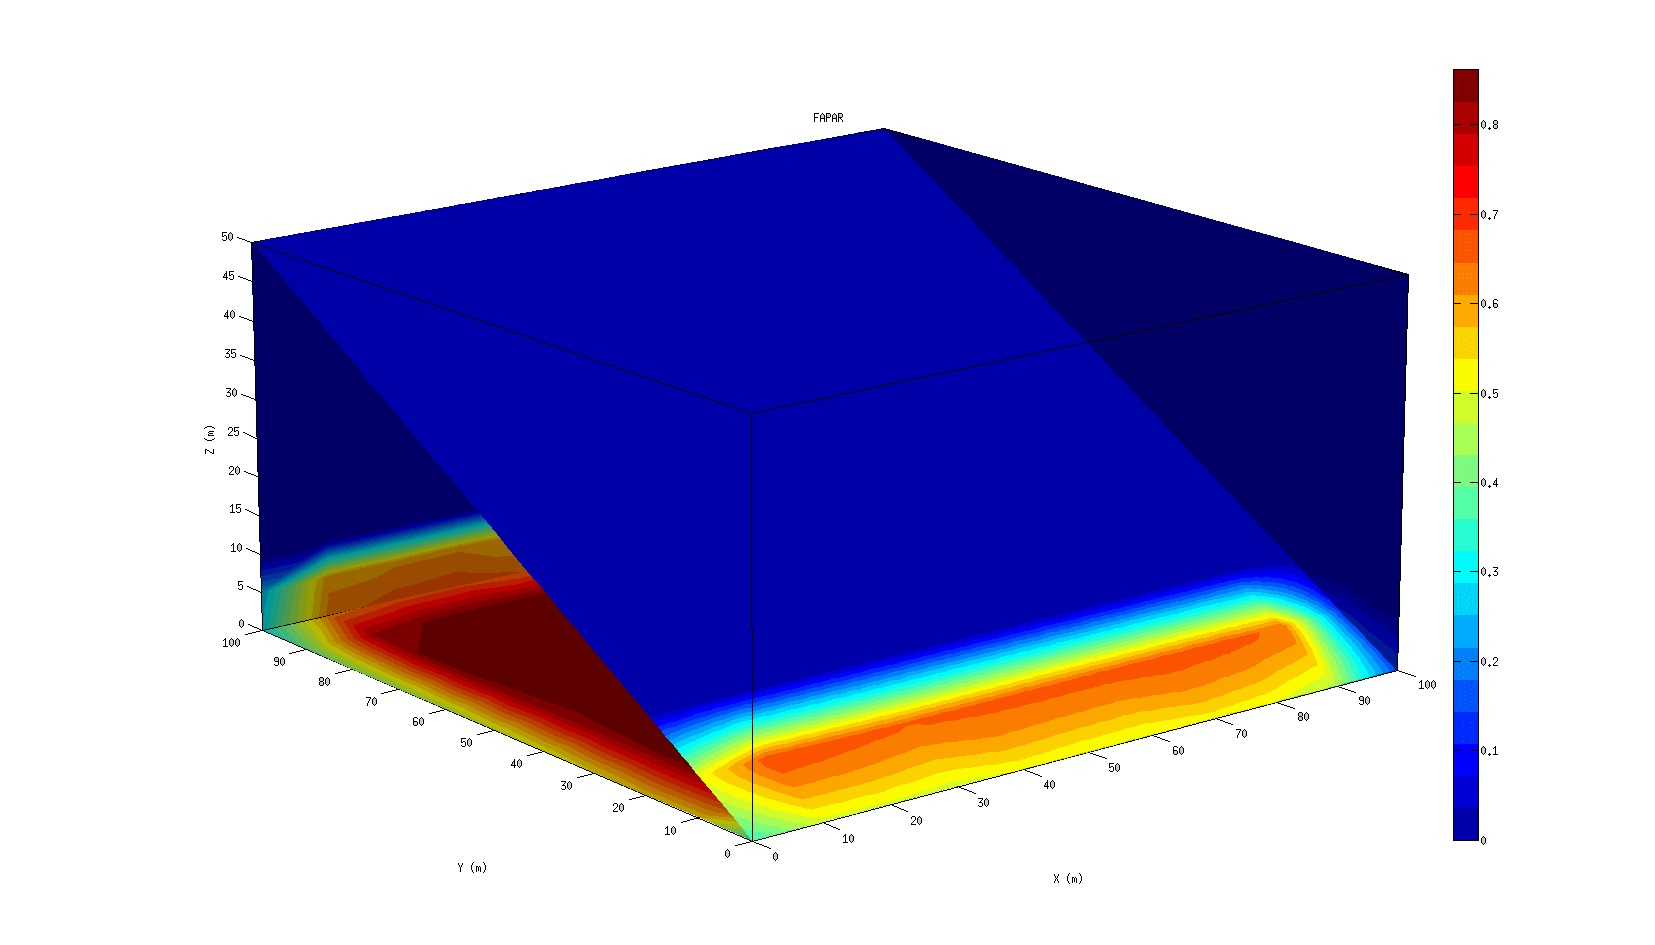
\includegraphics[width=0.6\textwidth]{/home/mn811042/Thesis/chapter4/figures/FAPAR_dense.png}}
\end{tabular}
\caption{One hectare (100 m x 100 m) of three different canopy densities: sparse, medium and dense. Red trees represent target trees, i.e., trees reached by radiation (left); 3D profile of PAR absorption (right).}
\label{f:3d_maespa}
\end{figure}

Fig.~\ref{f:3d_maespa} shows a 3D representation of each one of the three canopy densities, where red trees indicate the target trees. The selection of randomly distributed target trees within a vegetation canopy is a method implemented to save computational time when running a complex 3D tree based model like MAESPA, but without compromising the final results. 

As MAESPA calculates the radiative balance, water balance and surface energy balance for each single tree present in the canopy, the amount of computational time spend in a very dense canopy can be relatively long. Using fewer target trees for complete flux calculations and surrounding trees when calculating the mutual crown shading of the target tree does not alter the final results in radiation absorption, as evaluated in edge experiments. 

The 3D profile of PAR absorption can be spatially different for each one the three canopy densities, even though the LAI is constant between them (3.2 m$^2$.m$^{-2}$). For the sparse case, few tree crowns are responsible for large amounts of absorbed radiation with several spots with no absorption at all, especially at the bottom of the canopy. For the dense case, radiation absorption behaves almost uniformly within the 3D space, with larges values at the centre and top of the canopy. The border effect plays a role here once the canopies are finite and radiation is direct. The borders show less absorption because of lower scattering. 

The same LAI value was used in JULES under two different sky conditions: totally diffuse light (TS isotropic) and direct light (TS direct). Under an isotropic illumination condition, the JULES output value of fraction of absorbed photosynthetically radiation (fAPAR) is constant (fAPAR ~ 0.9) with solar zenith angle. For direct illumination, the fAPAR varies from 0.77 to 0.93 and it is systematically lower than the diffuse condition until a solar zenith angle of approximately 60$^{\circ}$ (Fig.~\ref{f:ts_maespa}). In comparison to MAESPA (isotropic illumination condition), both JULES scenes are overestimating the fAPAR values, which indicates that 3D representations are more transparent than their 1D equivalent with respect to the direct transmitted radiation. Although, for a dense canopy under illumination angles between 0$^{\circ}$ and 40$^{\circ}$, fAPAR values obtained by MAESPA and JULES TS direct are comparable. That shows an accurate performance of JULES in partitioning PAR in densely vegetated canopies, such as tropical rainforests, for example. However, in sparser canopies with same LAI, the TS method seems to overestimate fAPAR in 25\% for medium vegetated canopies and up to 50\% for sparse vegetated canopies. 

\begin{figure}
\centering
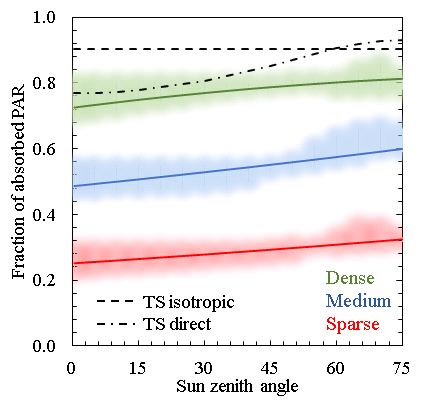
\includegraphics[width=0.5\textwidth]{/home/mn811042/Thesis/chapter4/figures/fAPAR_sza.png}
\caption{Fraction of absorbed photosynthetically active radiation (PAR) with respect to the JULES Two-Stream method (black lines) for a diffuse isotropic case (dashed line) and for a direct illuminated case (dash-dotted line). The colour lines represents three different vegetation canopies in MAESPA, described in Table~\ref{tab:parameters_laisense}. The illumination condition was an overcast sky and the shaded areas are associated with azimuth variations. The LAI is 3.2 m$^2$.m$^{-2}$ for all scenarios.} 
\label{f:ts_maespa}
\end{figure}

\section{Considering structural effects in 1D radiative transfer treatments}
Several previous studies have suggested with observations and detailed modelling approaches that vegetation three-dimensional (3D) structure influences radiation partitioning and other land surface related processes \citep{Nilson1971,Wang1990,Chen1996,Kucharik1999,Yang2001,Yang2003,Jonckheere2004,pinty2006,Chen2008,Ni-Meister2010,Widlowski2011,Kobayashi2012,Loew2014}. For most natural woody vegetation, such as conifers and savannahs, the spatial distribution of individual tree crowns creates clear spaces whereas beam radiation propagates without interference of vegetation elements, and the two-stream approximation (vertical 1D) results in large deviations from the actual amounts of absorbed and reflected radiation \citep{Ni-Meister2010,Kobayashi2012,Loew2014}.

For detailed computation of 3D radiation fields within vegetation canopies, the models can have a geometrical optical approach and treat mixtures of individual trees, and multiple scattering with foliage clumped within tree crowns, e.g. in the GORT model \citep{Li1995}, or heterogeneously between tree crowns, e.g. in MAESTRA/MAESPA \citep{Wang1990,Duursma2012}, however these models cannot be directly applied into GCMs due to their extreme computational power demand \citep{Yang2001} and the high number of required vegetation structural parameters \citep{Loew2014}. 

Even though efficient 1D radiative transfer models are still preferably used, the use of effective radiative state variables to express the properties of 3D vegetation canopy systems makes a simpler model to analogously simulate the radiation balance of more complex 3D models \citep{Pinty2004,pinty2006}. This requirement is not specific to vegetation canopy systems, but can be applied to every structurally heterogeneous radiative medium (i.e. clouds).

The probability of the transmission of a beam light through a vegetation canopy has been commonly described by the gap fraction (P$_{gap}(\theta)$) theory firstly proposed by \citet{Monsi1953,Monsi2005}: 
\begin{equation}
P_{gap}(\theta) = \exp{\Big(\frac{-G(\theta) \cdot LAI \cdot \Omega}{\cos{\theta}}\Big) = \exp{\Big(\frac{-G(\theta) \cdot L_e}{\mu}\Big)}
\label{equation:pgap}
\end{equation}
\noindent where P$_{gap}(\theta)$ is the direct transmittance, $\theta$ is the solar zenith angle, $\mu$ is the cosine of the solar zenith angle, G($\theta$) is the `G-funtion' \citep{Ross1981} defined as the leaf projection function on the plane perpendicular to the view direction \citep{WarrenWilson1960,Ross1981,Sellers1985,Myneni1989} and often assumed to be a spherical distribution of leaf normals \citep{Chen1992,Chen2012}, $L$ is the true LAI (leaf area index) and $\Omega$ is the `clumping index' firstly proposed by \citet{Nilson1971}, but revisited by many other authors to account for structural heterogeneities associated with the evaluated vegeation canopy. Therefore, $L_e$ is referred as the `effective LAI', a domain-averaged quantity, that can be forced to satisfy the main constraints associated with a 1D representation by any factor accounting for structural variabilities in a determined turbid medium.

Thus $L_e$ accounts for all phyto and woody elements composing the vegetation canopy, and when its value exceeds the true LAI, it is an indication of specific structural canopy conditions associated with significant amounts of woody elements \citep{pinty2006}. 

The `clumping index' \citep{Nilson1971,Norman1974,Chen1996} is associated with the heterogeneous nature of the canopy volume, often used at the tree resolution, and revisited later on by few authors \citep{Pinty2004,pinty2006}, who used the same scientific proposition to account for structural heterogeneities of different radiative media at stand scale, specially in association with sattelite products.

Few authors \citep{Kucharik1999,pinty2006,Ni-Meister2010} attempted to formulate simplified modelling approaches to resolve vegetation clumping at several levels of organisation, in order to address one major difficulty associated with radiative transfer in forest canopies all over the world.

\subsection{The structure factor parameterisation}
Among other parameterisations, the one proposed by \citet{pinty2006} presents a relatively ``self-sufficiency'', because it does not require any previous knowledge about vegetation structure, and because of that, it can be applied to any vegetation canopy. The values of the effective variables can be estimated by inverting a 1D radiative transfer model against the results obtained by a 3D model \citep{pinty2006}.

Previous studies reported the dependency of the 'clumping index' on solar zenith angle \citep{Andrieu1993,Chen1996,Kucharik1999,Leblanc2005,Ryu2010}, and because this dependency remains rather smooth and limited (for dense boreal forest canopies with $\theta >$ 30$^{\circ}$) \citep{Chen1997a,Chen1997}, it was re-written by \citet{pinty2006} so it can be approximated by a linear relationship:
\begin{equation}
\Omega = \zeta(\mu) \approx a + b \cdot (1 - \mu)
\label{equation:structurefactor}
\end{equation}
\noindent where $\mu$ is the cosine of $\theta$, $a = \zeta(\mu=1)$ is the parameter corresponding to an overhead Sun, and $b$ the parameter responsible for include the effects of a range of different Sun geometries.

In the particular case of an overhead Sun ($\theta$ = 0$^{\circ}$), $a$ is also equal to:
 \begin{equation}
\zeta(\mu=1) = -\ln{(1 - F_c)}\frac{2}{LAI}
\label{equation:structurefactora}
\end{equation}
\noindent where $F_c$ is the true (within and between crown gaps) vegetation cover obtained for a Black Canopy representation ($\rho_{leaf} = \tau_{leaf} = 0.0$) of the total incident radiation minus direct transmissivity with an overhead Sun (1 - P$_{gap}(\theta = 0^{\circ}$)).
Both parameters are used to account for vegetation canopy heterogeneities and correctly simulate the radiation path length. 

The structure factor is introduced into the two-stream approximation by modifying three main groups of variables to account for canopy structural effects:
\begin{enumerate}
\item the optical depth of direct beam per unit leaf area, $K$; 
\item the average inverse diffuse optical depth per unit leaf area, $\mu$̅; and, 
\item the single scattering albedo, $a_s(\mu)$, used to obtain the upscattering parameters for the diffuse and direct beams, $\beta$ and $\beta_0$.
\end{enumerate}
The structure factor can be included on the optical depth of direct beam per unit leaf area, $K$, by simply:
\begin{equation}
K_{Structure}(\theta) = \frac{G(\theta)}{\mu} \cdot  \zeta(\mu)
\label{equation:opticaldepthstruct}
\end{equation}
The same analogy can be applied when calculating the average inverse diffuse optical depth per unit leaf area, $\bar{\mu}$, but obtaining the structure factor for the direction of scattered flux, $\mu^\prime$:
\begin{equation}
\overline{\mu_{Structure}} = \int_{0}^{1} \frac{\mu^\prime}{G(\mu^\prime) \cdot \zeta(\mu^\prime)} d\mu^\prime
\label{equation:muprimestruct}
\end{equation}
The parameter $\omega\beta$ can be inferred from the analysis of \citet{Norman1975} in the case of a single leaf whose normal is oriented at zenith angle $\theta_l$ from the local vertical defined in the upward hemisphere:
\begin{equation}
\omega\beta = \frac{1}{2}(\omega_l + \delta_l \cos^2 \theta_l)
\label{equation:omegabeta}
\end{equation}
\noindent where $\omega_l = \rho_{leaf} + \tau_{leaf}$ and $\delta_l = \rho_{leaf} - \tau_{leaf}$. 

The equation~\ref{equation:omegabeta} however is only valid for a single leaf and to obtain the total contribution of leaves over the canopy it is necessary to integrate over the appropriate leaf orientation probability distribution, between 0 and $\pi/2$, because the leaf normal are assumed to be oriented into the upward hemisphere, as in:
\begin{equation}
\omega\beta = \frac{1}{2}\Big(\omega_l + \delta_l \int_{0}^{\pi/2} \cos^2 \theta_l g^\prime(\theta_l) \sin \theta_l d\theta_l\Big)
\label{equation:omegabeta2}
\end{equation}
\noindent where $\sin\theta_l$ is introduced for normalisation requirement of the probability distribution function. And when isolating $\beta$, it is possible to obtain the generic diffuse upscatter parameter:
\begin{equation}
\beta = \frac{1}{2\omega}\Big(\omega_l + \delta_l \int_{0}^{\pi/2} \cos^2 \theta_l g^\prime(\theta_l) \sin \theta_l d\theta_l\Big)
\label{equation:beta}
\end{equation}
If the two-stream scheme equations are solved when $\omega \varinjlim 0$, i.e., single scatter approximation and semi-infinite canopy, the upward diffuse flux at the top of the canopy may be taken as equal to the single scattering albedo ($a_s(\mu)$). The equation for the direct upscatter parameter, $\beta_0$, is
\begin{equation}
\beta_0 = \frac{1 + \overline{\mu}K}{\omega\overline{\mu}K}a_s(\mu)
\label{equation:betazero}
\end{equation}
And $a_s(\mu)$ is given by, 
\begin{equation}
a_s(\mu) = \frac{\omega}{2}\int_{0}^{1} \frac{\mu^\prime G(\mu)}{\mu G(\mu^\prime) + \mu^\prime G(\mu)} d\mu^\prime
\label{equation:alphas}
\end{equation}
The above equation is just valid when assuming isotropic scattering for the leaf elements, which makes the scattering phase function independent of the angle of the incident beam (see \citet{Dickinson1983} and \citet{Sellers1985} for more details). The addition of the structure factor into the single scattering albedo formulation would result in,  
\begin{equation}
a_s(\mu) = \frac{\omega}{2}\int_{0}^{1} \frac{\mu^\prime G(\mu) \zeta(\mu)}{\mu G(\mu^\prime) \zeta(\mu^\prime) + \mu^\prime G(\mu)\zeta(\mu)} d\mu^\prime
\label{equation:alphasstruct}
\end{equation}
In this case the formulation for the direct upscatter parameter considering canopy structure would be: 
\begin{equation}
\beta_0 = \frac{1 + \overline{\mu_{Structure}}K_{Structure}}{\omega\overline{\mu_{Structure}}K_{Structure}}
\bigg[\frac{\omega}{2}\int_{0}^{1} \frac{\mu^\prime G(\mu) \zeta(\mu)}{\mu G(\mu^\prime) \zeta(\mu^\prime) + \mu^\prime G(\mu)\zeta(\mu)} d\mu^\prime \bigg]
\label{equation:alphasstruct}
\end{equation}

\subsection{The clumping index by Kucharik et al. (1999)}
The first study evaluated in this section was developed by \citet{Kucharik1999}. The authors used measurements of LAI and gap fraction made with MVI (Multiband Vegetation Imager) \citep{Kucharik1997} obtained during the BOREAS (Boreal Ecosystem-Atmosphere Study) \citep{Sellers1997} field campaigns of 1994-1996 to derive a semi-empirical \citep{Ni-Meister2010} relationship between $\Omega(\theta)$ and zenith angle ($\theta$). In this method, two key quantities are needed: (i) the fraction of ground area covered by the horizontal projection of crown envelopes ($f_c$) (from nadir view), which is a function of the typical tree crown diameter ($D$), and tree stem spacing ($\lambda$), or stem density, within a study plot; and (ii) an estimate of crown porosity ($\Phi$); this quantity is related to foliage density and defined as the gap fraction within crown envelopes divided by $f_c$.
 
A series of zenith gap fraction measurements were needed along a transect beneath a canopy to partition the total gap fraction ($f_{gap},t(0)$) between within-crown and between-crown gaps, and  an estimate of the total fraction of ground area covered by the horizontal projection of crown envelopes ($f_c$). To obtain $f_c$, the typical crown silhouette area ($\pi r_c^2$, where $r_c$ is the crown radius in the horizontal direction) is multiplied by the number of crowns and divided by the total ground unit area on which the stem density is based. If $f_c$ is greater than 1, crowns typically overlap in the forest, and the entire value of fgap,t(0) can be defined as within-crown gap fraction ($f_{gap},c(0)$). The total gap fraction occurring between-crowns ($f_{gap},b(0)$) can be estimated by $1 − f_c$, and $f_{gap},c(0)$ is therefore approximated by $f_{gap},t(0) − f_{gap},b(0)$. If the value of $f_{gap},c(0) < 0$, it can be assigned a value of 0 for all practical purposes. 

Crown porosity ($\Phi$) is determined by dividing $f_{gap},c(0)$ by $f_c$ ($\Phi$ = $f_{gap},c(0)/f_c$). The value of $\Phi$ may be described as a normalised within-crown gap fraction. Generally, an error of about 0.05 exists in determining $f_c$ and $\Phi$ by using an average crown radius and tree stem density rather than the actual model calculations of $f_c$. However, the authors indicated that these errors are not of concern when estimating $\Omega(0)$ using the gap-fraction partitioning strategy.

Values of $\Phi$ and $f_c$ were then used to determine a value of $\Omega$(0) that was consistent with calculations resulting from numerical simulations of the canopy gap-size distribution. A nonlinear least-squares fit to approximately 250 Monte Carlo simulations (analysing values of $\Omega(0)$) was performed for values of $f_c$ $\geq$ 0.20, and for all simulated values of $\Phi$. A separate fit to the entire set of model data was performed for 0.04 $\geq f_c \geq$ 0.30. For sparse canopies where $f_c < 0.20$, a value of $\Omega(0)$ could still be determined. 

Ten equations were solved simultaneously to determine 10 coefficients ($a_0$,...,$a_9$) that describe the relationship between values of $\Omega(0)$, $f_c$, and $\Phi$. To characterise the angular dependence of $\Omega(\theta)$, a minimum value of $\Omega(\theta)$ was determined at $\theta$ = 0$^{\circ}$ and a value of $\Omega(\theta)$ was needed at $\theta$ = 90$^{\circ}$. Because it was assumed that $\Omega(\theta)$ reaches its maximum value at $\theta$ = 90$^{\circ}$, \citet{Kucharik1999} refer to this value as the maximum possible element clumping index, Ωmax, and defines it as:
\begin{equation}
\Omega_{max} = \Big(\frac{ND}{\sqrt{A}}\Big)^{0.7}
\label{equation:clumpmax}
\end{equation}
\noindent where $N$ is number of stems within ground area $A$, and $D$ is crown diameter. If $ND/\sqrt{A} > 1$, then the value of $\Omega_{max} = 1$. The angular dependence of $\Omega(\theta)$ was defined by Kucharik’s following equation: 
\begin{equation}
\Omega(\theta) = \frac{\Omega_{max}}{[1 + b\exp(-k(\theta)^p)]}
\label{equation:clumptheta}
\end{equation}
\noindent where $k$ is constant (usually $k$ = 2.2), $\theta$ is zenith angle expressed in radians, and $b$ is solved from a rearrangement of Eq.~\ref{equation:clumptheta} using a known value of $\Omega(\theta)$ (e.g., $\theta$ = 0$^{\circ}$). A quantitative comparison of results produced using Eq.~\ref{equation:clumptheta} with the best-fit curves suggested that a value for p can be approximated by an equation on the form:
\begin{equation}
p = -0.461\chi + 3.8
\label{equation:pchi}
\end{equation}
\noindent where $\chi$ is the ratio of crown depth to crown diameter. Generally, if $\chi$ is $\leq$ 1.0, $p$ = 3.34. 

This set of semi-empirical equations was used to estimate clumping index for three different canopy sets as in RAMI4PILPS. The results calculated by Eq.~\ref{equation:clumptheta} are presented by dotted lines in Fig.~\ref{f:ci_comparisons}. The authors also presented the best fit to data for each forest site by solid lines in the same figure. The range of clumping index obtained by this work was from approximately 0.2, for minimum Sun zenith angle (i.e. $\theta = 0^{\circ}$), with convergence to 1, for maximum Sun zenith angle (i.e. $\theta = 90^{\circ}$), for sparse and dense canopies, while the convergence for the medium canopy was approximately 0.7.

\subsection{The clumping index by Ni-Meister et al. (2010)}
Following the same attempt to derive a relationship for clumping index, \citet{Ni-Meister2010} developed an analytical prognostic expression based on stem density ($\lambda$), crown radius ($r$) and LAI. In here, only the formula used for sphere crowns is shown, however, the same authors extend the analysis to more generalised ellipsoid crowns, as introduced in \citet{Li1988}. The analytical solution for the modified clumping index in Beer$^{\prime}$s law is expressed as, 
\begin{equation}
\Omega = \frac{3}{4\tau_0r}\Big(1 - \frac{1 - (2\tau_0r + 1)\exp(-2\tau_0r)}{2\tau_0^2r^2}\Big)
\label{equation:clumpNi}
\end{equation}
\noindent where $\tau_0r = 3 G LAI/ 4 \lambda \pi \cdot r^2$ for spherical crowns. 

The authors compared the analytical solutions for clumping factor with the ones calculated by the full GORT model \citep{Li1995}, which was specifically developed to describe the effects of 3D canopy structure on the radiative balance and to characterise the heterogeneous radiative balance in natural vegetation at the forest stand scale. This set of equations was used to estimate clumping index for three different canopy sets as in RAMI4PILPS as well. The results calculated by Eq.~\ref{equation:clumpNi} are presented by dashed-dotted lines in Fig.~\ref{f:ci_comparisons}. The canopy sets are defined in such a way (LAI increasing with density), that the resulting clumping index stayed constant for all cases. 

\section{Evaluating structural parameterisations}
Evaluating model approaches is usually a challenge, specially when the study is designed to focus on fine details, e.g. different structural properties impacting radiation partitioning \citep{Kobayashi2012}. There are different ways to evaluate the performance of a specific radiative transfer scheme, including comparisons against different sources of observed data, such as bidirectional reflectance \citep{North1996,Malenovsky2008}, transmittance measurements at stand scale in various levels \citep{Norman1983,Wang1990,Tournebize1995,Law2001a,Sinoquet2001}, and gap fraction measurements \citep{Cescatti1997,Kucharik1999,Yang2010}. The use of field data is often limited and in order to eliminate uncertainties arising from an incomplete or erroneous knowledge of the structural, spectral and illumination related canopy characteristics typical of model comparisons with in-situ observations,  model-model intercomparison exercises have been used \citep{Pinty2001,Pinty2004,Widlowski2007,Widlowski2011,Widlowski2013}.

In special, the RAMI4PILPS \citep{Widlowski2011} was designed to evaluate the accuracy and consistency of shortwave radiative transfer formulations as used in GCMs by evaluating different models against the extensively verified 3D reference Monte Carlo model, raytran \citep{Govaerts1995} under perfectly controlled conditions.

In this evaluation only the RAMI4PILPS heterogeneous canopy scenario was used, where tree crowns were approximated by woodless spheres in an open forest canopy scene. Details of the RAMI4PILPS experiments used in the present study are summarised in Table~\ref{tab:RAMI4PILPS} and a graphic representation of the experiment setups can be found in Fig.~\ref{fig:rami}, while further details of the RAMI4PILPS experiments can be found in \citet{Widlowski2011}. 

For each scenario, simulations for different leaf area index and varying soil brightness are performed, assuming direct insulation for three different sun zenith angles as well as isotropic illumination conditions.

In a first analysis, the participant parameterisations were compared in two different ways:
\begin{enumerate}[i]
 \item by evaluating the behaviour of the structural index varying with Sun zenith angle, and
 \item by calculating the direct transmissivity ($P_{gap}$) through Eq.~\ref{equation:pgap}.
\end{enumerate}

\begin{threeparttable}
\centering
\caption{Summary of variables defining structurally heterogeneous scenes (see \citet{Widlowski2011} for details). Different soil albedos are defined as BLK = black, MED = medium, SNW = snow.}
%\begin{tabular*}{\textwidth}{ l@{\extracolsep{\fill}}*{4}{c}}
\begin{tabular}{l{0.25\textwidth} l{0.75\textwidth}}
%\begin{tabular}{\textwidth}{|p{\textwidth/4}|p{\textwidth/4}|p{\textwidth/4}|p{\textwidth/4}|}
%\begin{tabular*}
     \hline
     \hline
\textbf{Variable Identification}   & \textbf{Values (Units)}\\
\noalign{\smallskip}\hline
Leaf Area Index/ canopy	                & 0.50$^S$, 1.50$^M$ and 2.50$^D$ (m$^2$.m$^{-2}$)\\
Leaf Area Index/ sphere	                & 5.0$^S$, 5.0$^M$ and 5.0$^D$  (m$^2$.m$^{-2}$)\\
$1 – P_{gap} (\theta = 0^{\circ})$      & 0.09$^S$, 0.26$^M$ and 0.434$^D$\\
Tree density                            & 12.80$^S$, 38.24$^M$ and 63.68$^D$ (trees/hectare)\\
Maximum canopy height                   & 16 m\\
Minimum sphere centre height	        & 7 m\\
Maximum sphere centre height	        & 11 m\\
$\alpha_{soil},PAR / \alpha_{soil},NIR$	& BLK: 0.00/0.00; MED: 0.12/0.21; SNW: 0.96/0.56\\
Soil scattering law	                & Lambertian\\
$\rho_{leaf},PAR / \rho_{leaf},NIR$     & 0.0735/0.3912\\
$\tau_{leaf},PAR / \tau_{leaf},NIR$     & 0.0566/0.4146\\
Leaf scattering law                     & Bi-Lambertian\\
Sun zenith angle	                & 27.5/60.0/83.5/Isotropic(ISO)\\
Scatterer Normal Distribution           & Spherical\\
Woody area index                        & 0.0 (m$^2$.m$^{-2}$)\\
\hline
\hline%\noalign{\bigskip}
%\end{tabular*}
\end{tabular}
\begin{tablenotes}
      \small
      \item $^S$Sparse vegetation. $^M$Medium vegetation. $^M$Dense vegetation. 
\end{tablenotes}
\label{tab:RAMI4PILPS}
\end{threeparttable}
\bigskip

\begin{figure}
\centering
\begin{tabular}{lll}
\subfloat[Sparse Canopy]{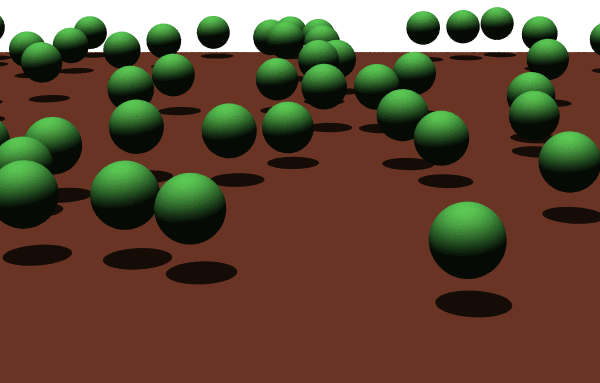
\includegraphics[width=0.33\textwidth]{/home/mn811042/Thesis/chapter4/figures/rami_lai_050.png}}
\subfloat[Medium Canopy]{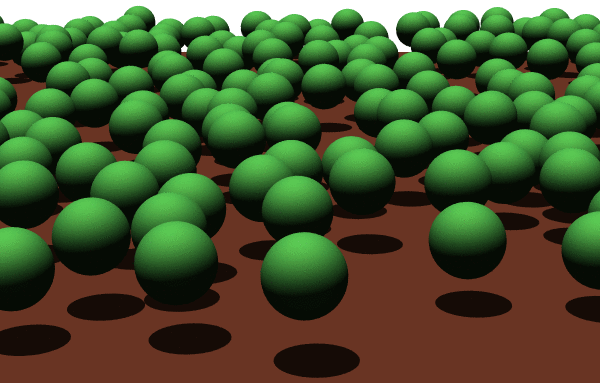
\includegraphics[width=0.33\textwidth]{/home/mn811042/Thesis/chapter4/figures/rami_lai_150.png}}
\subfloat[Dense Canopy]{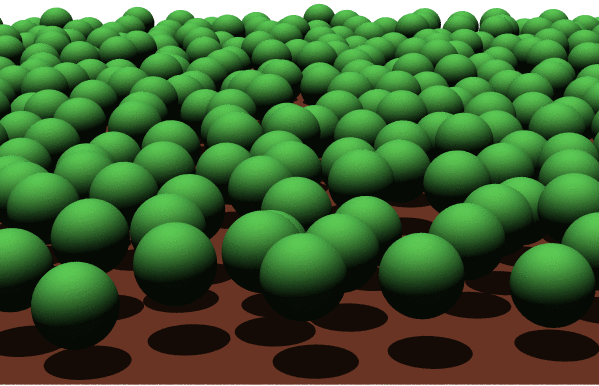
\includegraphics[width=0.33\textwidth]{/home/mn811042/Thesis/chapter4/figures/rami_lai_250.png}}
\end{tabular}
\caption{Graphical representation of the open forest canopy environments used in RAMI4PILPS. The images represent three different canopy structures \citep{Widlowski2011}.} 
\label{fig:rami}
\end{figure}

\begin{figure}
\centering
\begin{tabular}{ll}
\subfloat[Sparse Canopy]{\includegraphics[width=0.5\textwidth]{/home/mn811042/Thesis/chapter4/figures/CI_comparison_050.png}
                         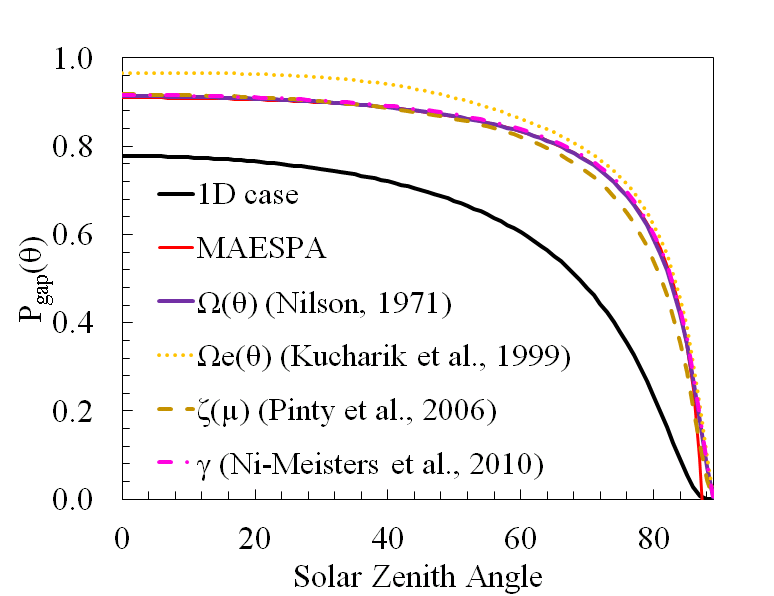
\includegraphics[width=0.5\textwidth]{/home/mn811042/Thesis/chapter4/figures/pgap_comparison_050.png}}
\end{tabular}

\begin{tabular}{ll}
\subfloat[Medium Canopy]{\includegraphics[width=0.5\textwidth]{/home/mn811042/Thesis/chapter4/figures/CI_comparison_150.png}
                         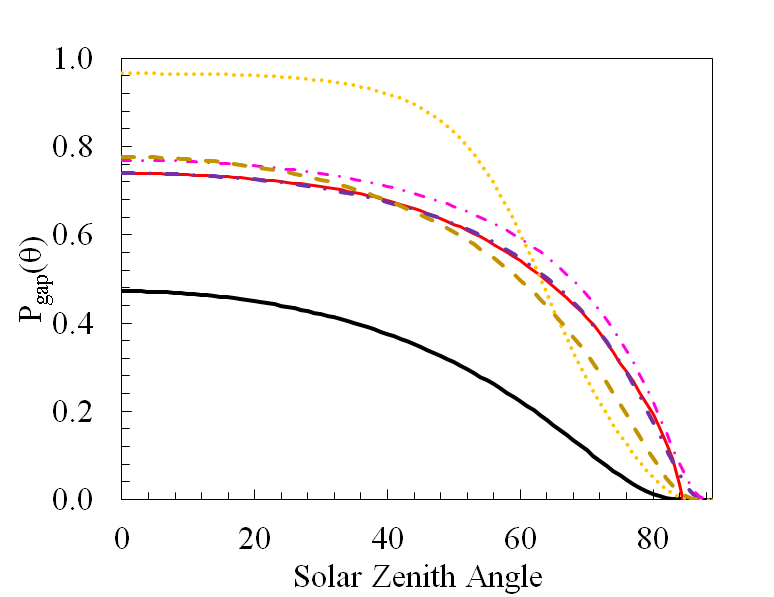
\includegraphics[width=0.5\textwidth]{/home/mn811042/Thesis/chapter4/figures/pgap_comparison_150.png}}
\end{tabular}

\begin{tabular}{ll}
\subfloat[Dense Canopy]{\includegraphics[width=0.5\textwidth]{/home/mn811042/Thesis/chapter4/figures/CI_comparison_250.png}
                        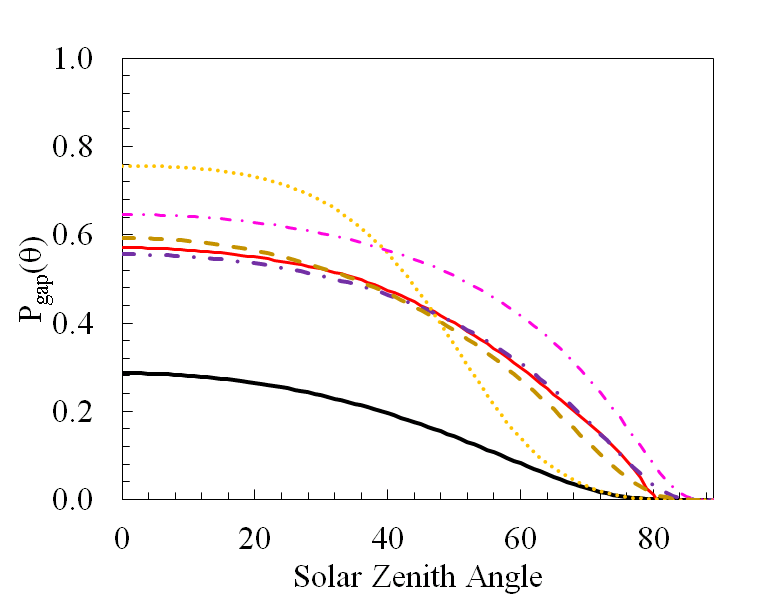
\includegraphics[width=0.5\textwidth]{/home/mn811042/Thesis/chapter4/figures/pgap_comparison_250.png}}
\end{tabular}

\caption{Comparison between different ways to calculate clumping index and its impact on gap fraction.}
\label{f:ci_comparisons}
\end{figure}

By following \citet{Kucharik1999}, it is necessary to know the number of stems within a pre-determined ground area, the crown diameter, and the ratio of crown depth to crown diameter. Besides that, Kucharik$^{\prime}$s relationship for determining clumping index is a semi-empirical equation adjusted for a specific set of data collected in boreal forests during the BOREAS large experiment. Its applicability could not necessarily be extended to other PFTs.

While in \citet{Ni-Meister2010}, the relationship for clumping index is based on an analytical prognostic expression, which can also just be determined with previous knowledge about stem density, crown radius and LAI. Besides that, the generalised equation for spheres does not depend on Sun zenith angle.

With the structure factor parameterisation, there is no need to have previous knowledge about canopy structure, whereas the parameters are minimised against calculated/measured terms of the radiation partitioning (absorbance, reflectance and/or transmittance). Results are summarised in Fig.~\ref{f:ci_comparisons}.

By comparing the gap probability generated by the three parameterisations with the one generated by the MAESPA model, the structure factor presented the lowest averaged RMSE (Fig.~\ref{fig:ci_rmse}).

\begin{figure}
\centering
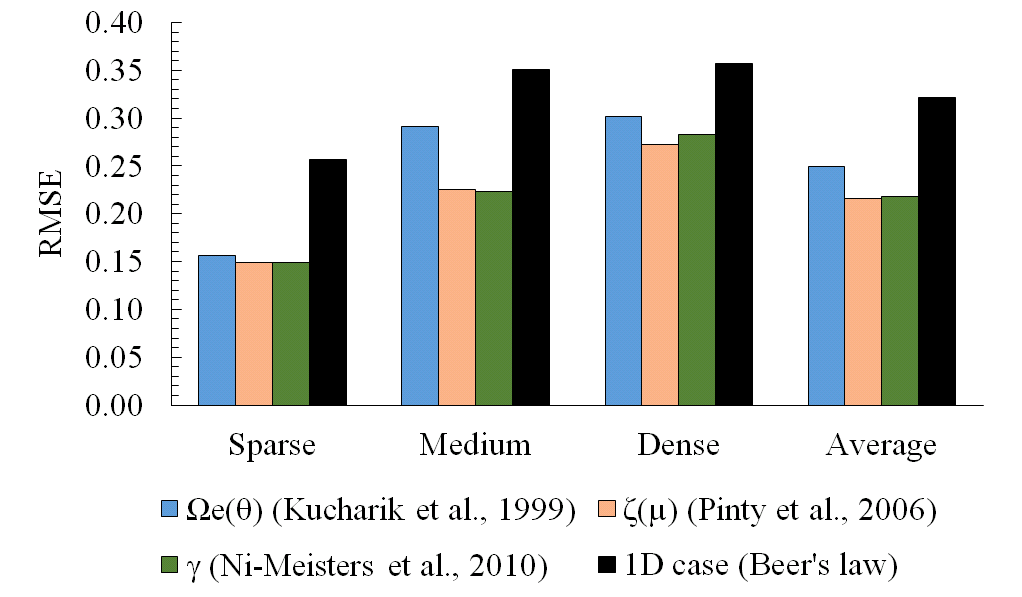
\includegraphics[width=1.0\textwidth]{/home/mn811042/Thesis/chapter4/figures/CI_rmse.png}
\caption{Root-Mean-Squared-Error of gap probability generated with three structural parameterisations and MAESPA for three different canopies densities (sparse, medium and dense) and the average.} 
\label{fig:ci_rmse}
\end{figure}

\subsection{Evaluating the structure factor parameterisation impacts on absorption and reflectance}
The structure factor parameterisation could be applied to any model, which the radiative transfer scheme is based on a two-stream approximation. The novelty about this parameterisation is its dependency on Sun zenith angle ($\theta$), which allows the parameterised scheme to account for geometric effects on the radiative balance, and the relative freedom of parameters, which are capable to reproduce more accurately the radiative balance of most of the vegetation canopies, for a variety of background albedos, under different shortwave radiation wavebands. 

A comparison between the performance of the structure factor parameterisation and state-of-art 3D radiative transfer schemes is conducted following a set of virtual scenarios described in the RAMI4PILPS experiment. For the present study, the participant models were used to simulate two flux quantities when available: 

(i) canopy absorption, which is defined as the fraction of radiation, entering the canopy via a virtual reference plane at the top‐of‐canopy height level, that has been absorbed by the elements in the scene, and 

(ii) canopy reflectance, which is defined as the ratio of reflected to incident radiation at the top‐of‐canopy level (spectral albedo), when available.

It is possible to determine the relative influence of both structure factor parameters $a$ and $b$ independently. A more rapid variation of fAPAR associate with a sun zenith angle of 27.5$^{\circ}$ following values of parameter $a$ on the x-axis indicates a relative larger impact of that variable than the one caused by the parameter $b$. Also, it is possible to conclude that a higher LAI is responsible for larger variations of fAPAR with the parameter $a$, represented by a more distinguishable variation in colours. 

For larger Sun zenith angles (60.0$^{\circ}$ and 83.5$^{\circ}$) the inclination of lines intervals towards the $b$ parameter gets stepper, which indicates an increase of the impact of parameter $b$ on the final result of fAPAR. 

Because $b$ is a parameter that modules angle variation as represented in Eq.~\ref{equation:structurefactor}, it is expect a more effective impact of $b$ on radiative transfer calculations for larger Sun zenith angles. A similar type of evaluation was conducted, but at this time instead of looking at a single Sun zenith angle, the average through all possible Sun zenith angle has been taken into account. To evaluate the sensitivity of the $structure factor$ parameters in JULES radiative transfer scheme in respect to canopy density, a minimum error evaluation was conducted varying $a$ and $b$ from 0 to 1 following the equation:
\begin{equation}
RMSE_{ab} = \sqrt{\frac{\sum_{n=1}^{N} (f_{Two-stream} - f_{MAESPA})^2}{N}}
\label{equation:rmseab}
\end{equation}
\noindent N = 90$^{\circ}$, $a$ = [0,1], $b$ = [0,1] and $f_{Two-stream}$ is the fAPAR calculated with the Two-stream radiative transfer scheme with the structure factor parameterisation for a combination of $a^{\prime}s$ and $b^{\prime}s$ and  $f_{MAESPA}$ is the fAPAR reference value calculated with the MAESPA model for different Sun zenith geometries varying from 0 to 90$^{\circ}$. MAESPA has been validated and it is a robust tool to calculate PAR absorption for different vegetation canopies, as it strongly agreed with the RAMI4PILPS reference values. 

The results showed in Figure~\ref{f:rmsd_ts_maespa} are limited to the PAR spectrum with a medium value of background albedo ($\alpha_{soil} = 0.12$). For all evaluated cases the combination of $a$ and $b$ that gives the minimum error between the 1D and the 3D cases is not a single value, but a combination of values described by a certain area of minimum Root-Mean-Squared-Erros (RMSE). This finding suggests that for a determined forest stand there are several combinations of  $a^{\prime}s$ and $b^{\prime}s$ that corrects the radiative transfer calculations of a 1D model and makes it matches with more complex 3D models. The sparse case seem to be equally sensitive to $a^{\prime}s$ and $b^{\prime}s$ parameters. As the canopy density increases, the sensitivity of a starts to increase in relation to $b$, as it can be noticed by the larger error variation on the axis of $a$. This indicates that for denser canopies b has reduced impact on architectural effects on radiation partitioning, if compared to $a$.

\begin{figure}
\centering
\begin{tabular}{lll}
\subfloat[LAI = 0.5 m$^2$.m$^{-2}$]{\includegraphics[width=0.33\textwidth]{/home/mn811042/src/julesRT_struct_2/julesRT_struct/RMSD_JULESRT_v2_MAESPA_050.png}}
\subfloat[LAI = 1.5 m$^2$.m$^{-2}$]{\includegraphics[width=0.33\textwidth]{/home/mn811042/src/julesRT_struct_2/julesRT_struct/RMSD_JULESRT_v2_MAESPA_150.png}}
\subfloat[LAI = 2.5 m$^2$.m$^{-2}$]{\includegraphics[width=0.33\textwidth]{/home/mn811042/src/julesRT_struct_2/julesRT_struct/RMSD_JULESRT_v2_MAESPA_250.png}}
\end{tabular}
\caption{Root-Mean-Squared-Deviation for Two-stream scheme with the structure factor parameterisation and MAESPA for three canopies densities (sparse, medium and dense).}
\label{f:rmsd_ts_maespa}
\end{figure}

The structure factor parameters were obtained for each canopy structure through the inversion of Two-stream scheme against direct and diffuse fAPAR and albedo PAR reference values from the RAMI4PILPS experiment. The Nelder-Mead minimisation method \citep{Nelder1964}, or downhill simplex was used in the inversion process. 

The structure factor parameters were obtained for each canopy density through inversion of fAPAR and albedo PAR values together over three soil backgrounds all together and are summarised bellow:

\begin{threeparttable}
\centering
\caption{Summary of the structure factor parameters minimised against the absorption and reflectance reference values for PAR waveband.}
\begin{tabular*}{\textwidth}{ l@{\extracolsep{\fill}}*{4}{c}}
%\begin{tabular}{{0.33\textwidth} {0.33\textwidth} {0.33\textwidth}}
%\begin{tabular}{\textwidth}{|p{\textwidth/4}|p{\textwidth/4}|p{\textwidth/4}|p{\textwidth/4}|}
%\begin{tabular*}
     \hline
     \hline
\textbf{Variable}   & \textbf{$a$} & \textbf{$b$}\\
\noalign{\smallskip}\hline
$\zeta_{sparse}(\mu)$ & 0.344 & 0.096\\
$\zeta_{medium}(\mu)$ & 0.337 & 0.256\\
$\zeta_{dense}(\mu)$  & 0.418 & 0.206\\
\hline
\hline%\noalign{\bigskip}
%\end{tabular*}
\end{tabular*}
\label{tab:structureparameters}
\end{threeparttable}
\bigskip

The structure factor associated with the sparse canopy is the one that presents more differences in relation to the homogeneous case, as expected. The curve in Figure~\ref{f:ci_comparisons}a indicates that for the sparse canopy the sparse effective LAI is that differs most from the true LAI. The structure factor associated with medium canopy presents an intermediate behaviour. It behaves like a sparse canopy for solar zenith angles smaller than 30$^{\circ}$, and the values start to converge to the dense canopy structure factor function towards larger solar zenith angles. 

The structure factor associated with the dense canopy has roughly the same behaviour than the sparse one with solar zenith variations, however presenting higher values towards 1, which is the homogeneous case. Also, the differences between sparse and dense structure factor gets more prominent for higher solar zenith angles.

Figure~\ref{f:adjusstruc_min} shows a scatter plot between the RAMI4PILPS reference values (3D Monte Carlo reference model) and two groups of data generated with: (i) the default two-stream radiative transfer scheme , and (ii) the same scheme, but with the structure factor parameterisation (Structure factor), for absorption ($+$) and reflectance ($\bigcirc$), for different backgrounds reflectance (black, medium and snow), canopy structures (sparse, medium and dense) and wavebands, PAR (Fig.~\ref{f:adjusstruc_min}a) and NIR (Fig.~\ref{f:adjusstruc_min}b).

\begin{figure}
\centering
\begin{tabular}{lll}
\subfloat[PAR]{\includegraphics[width=0.33\textwidth]{/home/mn811042/Thesis/chapter4/experiment2/jules_rami_050.png}
               \includegraphics[width=0.33\textwidth]{/home/mn811042/Thesis/chapter4/experiment2/jules_rami_150.png}
               \includegraphics[width=0.33\textwidth]{/home/mn811042/Thesis/chapter4/experiment2/jules_rami_250.png}}
\end{tabular}

\begin{tabular}{lll}
\subfloat[NIR]{\includegraphics[width=0.33\textwidth]{/home/mn811042/Thesis/chapter4/experiment2/jules_rami_050_NIR.png}
               \includegraphics[width=0.33\textwidth]{/home/mn811042/Thesis/chapter4/experiment2/jules_rami_150_NIR.png}
               \includegraphics[width=0.33\textwidth]{/home/mn811042/Thesis/chapter4/experiment2/jules_rami_250_NIR.png}}
\end{tabular}
\caption{Evaluation of absorption ($+$) and reflectance ($\bigcirc$) (a) PAR and (b) NIR with the default Two-stream radiative transfer scheme in comparison with the RAMI4PILPS reference values (3D Monte Carlo reference values), for all evaluated PAR cases. The colous indicate different soil albedos: {\color{black}BLACK}, {\color{red}MEDIUM} and {\color{blue}SNOW}.}
\label{f:adjusstruc}
\end{figure}

The two-stream method regarding NIR absorption presents a persistent overestimate from values calculated with the 3D model, while the values obtained with the parameterised structure factor presents the opposite behaviour, a persistent underestimate. 

Regarding the NIR reflectance, or albedo NIR, both models (Two-stream vs. Structure factor parameterisation) shows good agreement with the 3D model, with the parameterisation indicating slight improvement. 

From this analysis it is possible to assume, without major misleading, that the inversion of the structure factor parameters regarding the spectrum PAR is also valuable for calculations in the later part of the shortwave spectrum, i.e., NIR. 

\begin{figure}
\centering
\begin{tabular}{ll}
\subfloat[PAR]{\includegraphics[width=0.5\textwidth]{/home/mn811042/Thesis/chapter4/experiment2/jules_rami_all.png}
               \includegraphics[width=0.5\textwidth]{/home/mn811042/Thesis/chapter4/experiment2/jules_rami_all_structure.png}}
\end{tabular}
\begin{tabular}{ll}
\subfloat[NIR]{\includegraphics[width=0.5\textwidth]{/home/mn811042/Thesis/chapter4/experiment2/jules_rami_all_NIR.png}
               \includegraphics[width=0.5\textwidth]{/home/mn811042/Thesis/chapter4/experiment2/jules_rami_all_NIR_structure_minimised_against_PAR.png}}
\end{tabular}
\caption{Evaluation of absorption ($+$) and reflectance ($\bigcirc$) with the default Two-stream radiative transfer scheme in comparison with the RAMI4PILPS reference values (3D Monte Carlo reference values), for all evaluated PAR cases. The colous indicate different soil albedos: {\color{black}BLACK}, {\color{red}MEDIUM} and {\color{blue}SNOW}.}
\label{f:adjusstruc_min}
\end{figure}

\section{Evaluating the performance of the structure factor parameterisation with 3D models}
The present study uses four different radiative transfer approaches, where two of them (i.e. GORT \citep{Li1995,Ni1997} and MAESTRA \citep{Wang1990,Medlyn2004,Medlyn2007} are 3D models using different theories to describe radiation propagation in vegetation canopies. The 1D canopy radiative transfer model used in here is based on the two-stream approximation \citep{Sellers1985}, which is widely used in GCMs, and it was isolated from the main body of the JULES code \citep{Best2011,Clark2011}. Finally, the fourth model is an adaptation of the two-stream approximation including the structure factor parameterisation \citep{pinty2006}. Also, in order to evaluate an approach often implemented in GCMs to account for sparse vegetated canopies heterogeneities, a simple correction based on the amount of vegetation cover ($f_{veg}$) on a model grid cell is applied.

\subsection{MAESTRA/MAESPA}
The MAESTRA model \citep{Wang1990,Medlyn2004,Medlyn2007,Duursma2012} represents a forest canopy as an array of tree crowns, whose positions and dimensions are specified. The radiation routines are described in detail by \citet{Wang1990}. The canopy consists of individual tree crowns, which are described by a basic shape (one of several shapes, including ellipsoids, cylinders and cones), length, height to crown base, and width (in x and y directions). Radiation calculations are performed only for a set of target crowns specified by the user. The distribution of leaf area within the target crown is specified, as is the leaf angle distribution. The target crown is divided into usually 60 grid points, and the radiation penetrating to each grid point is calculated for three wavebands (PAR, NIR and thermal infra-red, TIR) based on shading within the crown, shading by neighbouring trees, the location of the sun, and whether radiation is direct or diffuse. Direct, diffuse and scattered radiation are considered separately. Scattering of radiation is approximated following \citet{Norman1979}. Leaf area within crowns is assumed to be distributed randomly, or to follow a beta distribution in horizontal and/or vertical directions \citep{Wang1990}. At each grid point, leaf area is separated into sunlit and shaded leaf area (Norman, 1993). The model has previously been applied to study canopy carbon and water fluxes of $Picea sitchensis$ \citep{Wang1990}, $Pinus radiata$ \citep{McMurtrie1993}, $Betula pendula$ \citep{Wang1998}, and $Pinus taeda$ \citep{Luo2001}. 
Using an R (R Development Core Team, 2011) package, Maeswrap (Duursma, 2015), the 3D stand scenes were graphically reproduced in 3D.

\subsection{GORT} 
The GORT model was developed to describe the effects of three-dimensional canopy structure on the radiation environment and to characterize the heterogeneous radiation environment in natural vegetation at the forest stand scale \citep{Li1995}. Merging theory from geometric optics and radiative transfer, the GORT model treats vegetation canopies as assemblages of randomly distributed tree crowns of ellipsoidal shape. The tree crowns are filled with leaves that absorb and scatter radiation passing through the crown. Principles of radiative transfer are used in describing the multiple scattering of leaves inside crowns and the multiple scattering among crowns and the ground surface. The GORT model was extended by \citet{Ni1997} to include the vertical canopy gap probability profile.

\subsection{Two-Stream: JULES (the Joint UK Land Environment Simulator)} 
The JULES model is the UK community land surface model designed to be interfaced with the UK Met Office Unified Model by predicting fluxes of heat, water and carbon between the land surface and the atmosphere. It originates from the Met Office Surface Exchange Scheme (MOSES) \citep{Cox1999}, and it includes the TRIFFID (Top-down Representation of Interactive Foliage and Flora Including Dynamics) dynamic vegetation model \citep{Cox2001}. The physical basis of JULES is common to most of the land surface models and are described in details in \citet{Best2011} and \citet{Clark2011}.

JULES uses a number of layers with equally distributed LAI to calculate the radiative transfer in the canopy for direct and diffuse radiation separately. The leaves extinction properties are prescribed by leaf reflectance ($\rho_{leaf}$) and transmittance ($\tau_{leaf}$) in the PAR and NIR wavebands and canopy leaf angle distribution (spherical or horizontal). The amount of absorbed incident radiation at each layer is therefore determined by sun zenith angle, incident direct and diffuse radiation at the top of the canopy, and the leaves extinction coefficients. 

The two-stream approximation assumes that diffuse radiative fluxes are isotropic in the upward and downward directions. Supposing that the upper and lower leaf optical properties are identical, the two-stream approximation used to model radiative transfer in plant canopies is given in the following form \citep{Dickinson1983,Sellers1985}: 
\begin{equation}
\begin{gathered}
-\overline{\mu}(dI^{\uparrow})/dL + [1 - (1 - \beta)\omega]I^{\uparrow} - \omega \beta I^{\downarrow} = \omega \overline{\mu} K \beta_0 \exp{(-KL)},\\
-\overline{\mu}(dI^{\downarrow})/dL + [1 - (1 - \beta)\omega]I^{\downarrow} - \omega \beta I^{\uparrow} = \omega \overline{\mu} K (1-\beta_0) \exp{(-KL)}
\end{gathered}
\label{equation:ts}
\end{equation}
\noindent where $I^{\uparrow}$ and $I^{\downarrow}$ are the upward and downward diffuse radiative fluxes normalized by the incident flux respectively, $\mu$ is the cosine of the zenith angle of the incident beam, $K$ is the optical depth of direct beam per unit leaf area and is equal to $G(\mu)/\mu$, $G(\mu)$ is the relative projected area of leaf elements in the direction $cos^{-1}\mu$, $\overline{\mu}$ is the average inverse diffuse optical depth per unit leaf area and is equal to $\int_{0}^{1}[\mu^{\prime}/G(\mu^{\prime})]d\mu^{\prime}$, $\mu^{\prime}$ is the direction of scattered flux, $\omega$ is the scattering coefficient and is equal to $\rho_{leaf} + \tau_{leaf}$, and $L$ is the cumulative LAI. $\beta$ and $\beta_0$ are upscattering parameters for the diffuse and direct beams respectively (see \citet{Sellers1985} for details). 

\subsection{Vegetation cover approach}
More simplified approaches to handle sparse vegetated canopies have been implemented in GCMs and are widely used \citep{Loew2014}. Suppose a model grid cell with area A, which is assumed to be fully covered (100\%) by a particular plant functional type (PFT). In the case of sparser canopies like, e.g., savannahs, the area A is covered by a dominant PFT (usually taller trees), a second PFT, for example, understory vegetation (e.g. shrubs, grass), or bare soil. The total area A is thus defined as,
\begin{equation}
A = Veg_{fraction} + Under_{fraction}
\label{equation:area}
\end{equation}
\noindent where $Veg_{fraction}$ is the fractional coverage of the major PFT and $Under_{fraction}$ corresponds to to the soil surface.  If the $LAI_{total}$ is the LAI over the area A, the LAI correspondent to the area $Veg_{fraction}$ is 
\begin{equation}
LAI_{Veg_{fraction}} = \frac{LAI_{Total}}{Veg_{fraction}}
\label{equation:laivegfraction}
\end{equation}
\noindent where $LAI_{Veg_{fraction}} \geq LAI_{Total}$. The fAPAR correspondent to the new area can be calculated as, 
\begin{equation}
fAPAR_{Veg_{fraction}} = fAPAR(LAI_{Veg_{fraction}})\cdot Veg_{fraction}
\label{equation:faparvegfraction}
\end{equation}
And the correspondent albedo ($\alpha$) can be obtained as, 
\begin{equation}
\alpha_{Veg_{fraction}} = (\alpha(LAI_{Veg_{fraction}}) \cdot Veg_{fraction} + (1 - Veg_{fraction}) \cdot \alpha_{soil})
\label{equation:albedovegfraction}
\end{equation}

\subsection{Solar Zenith Angular evaluations}
MAESPA was shown to be a robust tool to calculate PAR absorption for different vegetation canopies, as it strongly agreed with the RAMI4PILPS reference values, especially over non-bright surfaces. Figure 13 a and b shows that overall, JULESStructure (red dashed line) consistently showed a good agreement to the RAMI4PILPS reference values (black crosses) under direct (Solar Zenith Angles from 0 to 90$^{\circ}$) and diffuse illumination (ISO stands for isotropic) conditions. It seemed to be an efficient and accurate tool to derive PAR absorptance and reflectance for all evaluated scenarios, with especial attention to its performance over brighter backgrounds (snow). This effect is particularly relevant for the radiative balance treatment in boreal regions in the presence of snow, where the shadowing induced by spatially distributed plant structures diminishes surface albedo in comparison with a closed-canopy/bare-snow scenario of identical cover fractions \citep{Viterbo1999}. JULESStructure presented a better agreement with the reference values than any other model for absorptance and reflectance over snow. 

Also evaluated in this study, the GORT model was developed to describe the effects of 3D canopy structure on reflectance in natural vegetation at the forest stand scale \citep{Ni1999}. The description of canopy structure in GORT is statistical, i.e., with minimum and maximum values of tree height, crown radius and tree density. The GORT model was also considered in this experiment, because it calculates albedo values, which are not directly obtained from MAESPA.

Also presented in this comparison study, the vegetation fraction correction ($JULES_{VegFraction}$) is a common approach applied to account for canopy gaps in operational radiative balance calculations. \citet{Loew2014} applied the correction by simply multiplying the fAPAR by the fraction of vegetation cover; however I assumed that the correct way to do it is by: first, calculating the fAPAR for the “concentrated LAI” in a smaller area, which is the LAI divided by the fraction of vegetation cover; then, with the correct LAI, the fAPAR is calculated with the new value, and the correction is proceeded by multiplying the new fAPAR by the fraction of vegetation cover. This 1D correction reproduces the absorptance and reflectance of more complex models for low Sun zenith angles ($< 30^{\circ}$) and non-reflective backgrounds ($\alpha_{soil} \approx 0.0$), but does not reproduce the complete angular variation associated with variables used to obtain the radiative balance. 

\begin{figure}
\centering
\begin{tabular}{lll}
\subfloat[Sparse]{\includegraphics[width=0.33\textwidth]{/home/mn811042/src/figures/fabs_PAR_050_BLK.png}
                  \includegraphics[width=0.33\textwidth]{/home/mn811042/src/figures/fabs_PAR_050_MED.png}
                  \includegraphics[width=0.33\textwidth]{/home/mn811042/src/figures/fabs_PAR_050_SNW.png}}
\end{tabular}
\begin{tabular}{lll}
\subfloat[Medium]{\includegraphics[width=0.33\textwidth]{/home/mn811042/src/figures/fabs_PAR_150_BLK.png}
                  \includegraphics[width=0.33\textwidth]{/home/mn811042/src/figures/fabs_PAR_150_MED.png}
                  \includegraphics[width=0.33\textwidth]{/home/mn811042/src/figures/fabs_PAR_150_SNW.png}}
\end{tabular}
\begin{tabular}{lll}
\subfloat[Dense]{\includegraphics[width=0.33\textwidth]{/home/mn811042/src/figures/fabs_PAR_250_BLK.png}
                 \includegraphics[width=0.33\textwidth]{/home/mn811042/src/figures/fabs_PAR_250_MED.png}
                 \includegraphics[width=0.33\textwidth]{/home/mn811042/src/figures/fabs_PAR_250_SNW.png}}
\end{tabular}
\caption{Solar zenith profile of fraction of direct and diffuse (ISO) absorbed PAR calculated with 6 different models. JULES$_{Structure}$ parameters were obtained for each canopy density through inversion of fAPAR and albedo PAR values together over three soil backgrounds (BLK = black, $\alpha_{soil}$ = 0.00; MED = medium, $\alpha_{soil}$ = 0.12; and SNW = snow, $\alpha_{soil}$= 0.96). The obtained values of each structure factor parameters are described in Table~\ref{tab:structureparameters}.}
\label{f:szacomparisonfPAR}
\end{figure}

\begin{figure}
\centering
\begin{tabular}{lll}
\subfloat[Sparse]{\includegraphics[width=0.33\textwidth]{/home/mn811042/src/figures/fref_PAR_050_BLK.png}
                  \includegraphics[width=0.33\textwidth]{/home/mn811042/src/figures/fref_PAR_050_MED.png}
                  \includegraphics[width=0.33\textwidth]{/home/mn811042/src/figures/fref_PAR_050_SNW.png}}
\end{tabular}
\begin{tabular}{lll}
\subfloat[Medium]{\includegraphics[width=0.33\textwidth]{/home/mn811042/src/figures/fref_PAR_150_BLK.png}
                  \includegraphics[width=0.33\textwidth]{/home/mn811042/src/figures/fref_PAR_150_MED.png}
                  \includegraphics[width=0.33\textwidth]{/home/mn811042/src/figures/fref_PAR_150_SNW.png}}
\end{tabular}

\begin{tabular}{lll}
\subfloat[Dense]{\includegraphics[width=0.33\textwidth]{/home/mn811042/src/figures/fref_PAR_250_BLK.png}
                 \includegraphics[width=0.33\textwidth]{/home/mn811042/src/figures/fref_PAR_250_MED.png}
                 \includegraphics[width=0.33\textwidth]{/home/mn811042/src/figures/fref_PAR_250_SNW.png}}
\end{tabular}
\caption{Solar zenith profile of fraction of direct and diffuse (ISO) reflected PAR calculated with 6 different models. JULES$_{Structure}$ parameters were obtained for each canopy density through inversion of fAPAR and albedo PAR values together over three soil backgrounds (BLK = black, $\alpha_{soil}$ = 0.00; MED = medium, $\alpha_{soil}$ = 0.12; and SNW = snow, $\alpha_{soil}$= 0.96). The obtained values of each structure factor parameters are described in Table~\ref{tab:structureparameters}.}
\label{f:szacomparisonalbPAR}
\end{figure}

\begin{figure}
\centering
\begin{tabular}{lll}
\subfloat[Sparse]{\includegraphics[width=0.33\textwidth]{/home/mn811042/src/figures/fabs_NIR_050_BLK.png}
                  \includegraphics[width=0.33\textwidth]{/home/mn811042/src/figures/fabs_NIR_050_MED.png}
                  \includegraphics[width=0.33\textwidth]{/home/mn811042/src/figures/fabs_NIR_050_SNW.png}}
\end{tabular}
\begin{tabular}{lll}
\subfloat[Medium]{\includegraphics[width=0.33\textwidth]{/home/mn811042/src/figures/fabs_NIR_150_BLK.png}
                  \includegraphics[width=0.33\textwidth]{/home/mn811042/src/figures/fabs_NIR_150_MED.png}
                  \includegraphics[width=0.33\textwidth]{/home/mn811042/src/figures/fabs_NIR_150_SNW.png}}
\end{tabular}
\begin{tabular}{lll}
\subfloat[Dense]{\includegraphics[width=0.33\textwidth]{/home/mn811042/src/figures/fabs_NIR_250_BLK.png}
                 \includegraphics[width=0.33\textwidth]{/home/mn811042/src/figures/fabs_NIR_250_MED.png}
                 \includegraphics[width=0.33\textwidth]{/home/mn811042/src/figures/fabs_NIR_250_SNW.png}}
\end{tabular}
\caption{Solar zenith profile of fraction of direct and diffuse (ISO) absorbed NIR calculated with 6 different models. JULES$_{Structure}$ parameters were obtained for each canopy density through inversion of fAPAR and albedo PAR values together over three soil backgrounds (BLK = black, $\alpha_{soil}$ = 0.00; MED = medium, $\alpha_{soil}$ = 0.12; and SNW = snow, $\alpha_{soil}$= 0.96). The obtained values of each structure factor parameters are described in Table~\ref{tab:structureparameters}.}
\label{f:szacomparisonfNIR}
\end{figure}

\begin{figure}
\centering
\begin{tabular}{lll}
\subfloat[Sparse]{\includegraphics[width=0.33\textwidth]{/home/mn811042/src/figures/fref_NIR_050_BLK.png}
                  \includegraphics[width=0.33\textwidth]{/home/mn811042/src/figures/fref_NIR_050_MED.png}
                  \includegraphics[width=0.33\textwidth]{/home/mn811042/src/figures/fref_NIR_050_SNW.png}}
\end{tabular}
\begin{tabular}{lll}
\subfloat[Medium]{\includegraphics[width=0.33\textwidth]{/home/mn811042/src/figures/fref_NIR_150_BLK.png}
                  \includegraphics[width=0.33\textwidth]{/home/mn811042/src/figures/fref_NIR_150_MED.png}
                  \includegraphics[width=0.33\textwidth]{/home/mn811042/src/figures/fref_NIR_150_SNW.png}}
\end{tabular}

\begin{tabular}{lll}
\subfloat[Dense]{\includegraphics[width=0.33\textwidth]{/home/mn811042/src/figures/fref_NIR_250_BLK.png}
                 \includegraphics[width=0.33\textwidth]{/home/mn811042/src/figures/fref_NIR_250_MED.png}
                 \includegraphics[width=0.33\textwidth]{/home/mn811042/src/figures/fref_NIR_250_SNW.png}}
\end{tabular}
\caption{Solar zenith profile of fraction of direct and diffuse (ISO) reflected NIR calculated with 6 different models. JULES$_{Structure}$ parameters were obtained for each canopy density through inversion of fAPAR and albedo PAR values together over three soil backgrounds (BLK = black, $\alpha_{soil}$ = 0.00; MED = medium, $\alpha_{soil}$ = 0.12; and SNW = snow, $\alpha_{soil}$= 0.96). The obtained values of each structure factor parameters are described in Table~\ref{tab:structureparameters}.}
\label{f:szacomparisonalbNIR}
\end{figure}

\subsection{Vertical evaluation of the structure factor parameterisation}
The zenith profile of fAPAR calculated by the two-stream scheme overestimates the profiles obtained by the radiative transfer models with consideration of vegetation canopy spatial heterogeneities for nine experimental setups conducted in previous sections, three different canopy structures over three different soil albedos. By parameterising canopy structure following \citet{pinty2006}, it was possible to make the two-stream scheme matches the fAPAR zenith profile of a 3D Monte Carlo reference model \citep{Widlowski2011}. The previous evaluations, however, only considered the total canopy fAPAR with no vertical discrimination. 

The vertical profile of fAPAR in a vegetation canopy is important because it tells how the radiation is distributed along different canopy layers and in reality different vertical points in a vegetation canopy have different properties that will ultimately affect biogeophysical processes as photosynthesis, for example. 

The major source of vertical differences on PAR absorption along a vegetation canopy is the LAI distribution within the canopy. Although there are many possibilities for plants to distribute the LAI vertically, the most common one is an accumulation of leaves towards the top of the canopy where there is more light availability. 

In order to simplify the problem, before moving to the actual vertical comparison of fAPAR for the RAMI4PILPS canopy sets, a virtual black canopy (leaf reflectance,  transmittance and soil albedo set zero) with LAI = 1.0 m$^2$.m$^{-2}$  (Fig.~\ref{f:blackcanopy}) was evaluated. In a black canopy there is no scattering processes and because of that by following the energy conservation law, everything that is not absorbed in one particular wavelength is than transmitted. This simplification guarantees that all evaluated radiation is direct and isolates in a first instance the deviation between fAPAR values generated with the two-stream scheme and more detailed radiative transfer models only with respect to absorption. 

Figure~\ref{f:faparblackvertical} shows the vertical profile of fAPAR (1 - $P_{gap}$) for a black canopy (black leaves and black soil) with LAI = 1.0 m$^2$.m$^{-2}$ and vegetation cover 20\%. Both radiative transfer approaches agree for zenith angles of 27.5$^{\circ}$ and 60.0$^{\circ}$, however they disagree for the zenith angle of 83.5$^{\circ}$. GORT overestimates MAESPA absorption by up to 20\% at the bottom of the canopy. 

\begin{figure}
\centering
\includegraphics[trim=3.5cm 4cm 4cm 10cm,angle=0,clip=True,width=0.8\textwidth]{/home/mn811042/Thesis/chapter4/experiment3/blackcanopy/blackcanopy_100_000.png}
\caption{Graphical representation of an open forest canopy with LAI = 1.00 m$^2$.m$^{-2}$ and vegetation cover of 20\%. 160 black spheres distributed over 250 m x 250 m.}
\label{f:blackcanopy}
\end{figure}

\begin{figure}[ht!]
\centering
\begin{tabular}{lll}
\subfloat[Height]{\includegraphics[width=0.33\textwidth]{/home/mn811042/Thesis/chapter4/experiment3/blackcanopy/fapar_vertical_profile_100_000_27_height.png}
         \includegraphics[width=0.33\textwidth]{/home/mn811042/Thesis/chapter4/experiment3/blackcanopy/fapar_vertical_profile_100_000_60_height.png}
         \includegraphics[width=0.33\textwidth]{/home/mn811042/Thesis/chapter4/experiment3/blackcanopy/fapar_vertical_profile_100_000_83_height.png}}
\end{tabular}

\begin{tabular}{lll}
\subfloat[Layer]{\includegraphics[width=0.33\textwidth]{/home/mn811042/Thesis/chapter4/experiment3/blackcanopy/fapar_vertical_profile_100_000_27_layer.png}
                 \includegraphics[width=0.33\textwidth]{/home/mn811042/Thesis/chapter4/experiment3/blackcanopy/fapar_vertical_profile_100_000_60_layer.png}
               \includegraphics[width=0.33\textwidth]{/home/mn811042/Thesis/chapter4/experiment3/blackcanopy/fapar_vertical_profile_100_000_83_layer.png}}
\end{tabular}
\caption{Height vertical profile and b. Layer vertical profile of fAPAR (1 - P$_{gap}$) with LAI = 1.0 m$^2$.m$^{-2}$, vegetation cover of 20\% and $\alpha_{soil}$  = 0.0 for three zenith angles: 27.5$^{\circ}$, 60.0$^{\circ}$ and 83.5$^{\circ}$; and three different mathematical approaches: GORT (geometric optics), MAESPA (tree based) and Two-stream.}
\label{f:faparblackvertical}
\end{figure}

MAESPA and GORT are different on the way the virtual canopy is built. The tree based approach uses the exact position of each black sphere (160 in this case) distributed on the 3D space (x,y,z), and the geometric optics approach uses a mean distribution of spheres through the 3D space ($\lambda$: tree density (1/m$^2$), $h_1$: lower boundary of the crown centres, $h_2$: upper boundary of the crown centres). For higher zenith angles the optical depth of the canopy is bigger and GORT seems to absorb more radiation than MAESPA. A possible explanation for this behaviour might be related to the fact that the actual distribution of LAI calculated by the tree based model differs from the averaged one calculate by the geometric optics. GORT is seeing more LAI at the bottom layers. 

The Two-stream scheme overestimates both 3D models for all evaluated cases with major discrepancies for bottom layers and high zenith angles. This behaviour indicates that a possible way to correct the radiation absorption calculated by the Two-stream scheme would be a reduction of the total LAI value to correspond to the actual optical depth of a determined vegetation canopy. This correction factor dependents on angular variations of incident light, so it is valid to assume that it should be proportional to sun zenith angle.

\section{Summary of Findings}
produce noisy seasonal dynamics. However it was also suggested that even though the collection 5 product represented an improvement it also had a tendency to underestimate the highest LAI values. De Kauwe et al. (2011) argued that the lower level products such as the vegetation indices that undergo less processing may be more suitable for use in model validation studies because there are fewer underlying assumptions that may conflict with those inherent in a global vegetation model. Huete et al. (2011) consider vegetation index data to be a more accurate representation of the true surface measurements because the same algorithm is used regardless of biome type, land cover or soil type.

The uncertainties present in the MOD15 LAI/fPAR products also have implications for the MOD17 GPP product which relies on these data to make productivity estimates. A study assessing MODIS LAI by Jensen et al. (2011) using Lidar retrievals found that there were large differences in the performance of the MOD15 LAI product depending on which version of the retrieval algorithm had been implemented. This has implications for users of the data because for the main algorithm it was found that there is an underestimation of LAI which agrees with the findings of De Kauwe et al. (2011), this was further confirmed by Fang et al. (2012), however for the alternative algorithm there is trend towards overestimation of the LAI. The retrieval rate for the main algorithm of the LAI
product was found to be highest for grasses and crops and lowest for broadleaf forests. Retrieval rates for needleleaf forests in the boreal zone are seasonal due to snow cover and the solar zenith angle during the winter also reduces the retrieval rate in high northern latitudes (Myneni et al., 2011).

Fang et al. (2013a) compared 5 different satellite derived LAI products and found that overall the products all agreed with each other over the seasonality of LAI however the value of the LAI was often in disagreement with some products consistently higher or lower than the multi-product mean. The agreement between the products was strongest for grasses, crops, shrubs and savanna with a reduced level of agreement for forested areas. In general the uncertainty with all products is highest in forested regions and lowest in agricultural regions. The average LAI uncertainty for MODIS was 0.17 which gave it a relative uncertainty of 11.5\% when compared
to the other products and made it the product with the lowest overall uncertainty when all global measurements were averaged. The impact of errors in the MODIS land cover product on the quality of the LAI data was investigated by Fang et al. (2013b). It was found that the largest errors due to land cover misclassifcation were for savannas because they were often misclassified as grasses, crops or shurbs. There are also problems with the misclassification of the four dominant forest types. The total number of high confidence pixels across the globe where only a single vegetation type is present is 0.92\% (Fang et al., 2013b) with the remainder of the land surface being composed of mosaics of two or more vegetation types which means that misclassification is always going to be a problem for all land cover products and not just the MODIS data sets.

The initial validation of the MODIS NDVI and EVI products by Huete et al. (2002) found that the NDVI was prone to saturation in densely vegetated regions such as the Amazon but the EVI was still sensitive to changes in vegetation cover. They also found that seasonal phenology was captured well for a range of ecosystems in North and South America and indicated that the quality of the data from the MODIS sensor was of a higher quality than the AVHRR NDVI data set. An investigation into the sensitivity of MODIS NDVI and EVI to the effects of topography by Matsushita et al. (2007) found that the soil adjustment factor (L in equation 3.8) used in the EVI algorithm makes it more sensitive to topographic effects than the NDVI. This effect is related to the scale of
